\documentclass[oneside,11pt,dvipsnames]{book}

\usepackage[utf8]{inputenc}
\usepackage[T1]{fontenc}
\usepackage[margin=1.5in]{geometry}
\usepackage{soul}
% \usepackage[small,compact]{titlesec} %very powerful
\usepackage[most]{tcolorbox}
% \setsecnumdepth{subsection}
% \setcounter{tocdepth}{3}
\usepackage{enumitem}
\usepackage{epigraph}
\usepackage{cite}
\usepackage{caption}
\captionsetup{font=small}
\usepackage{graphicx}
\usepackage{pdfpages}
\usepackage{hyperref}
\usepackage{wrapfig}
\setlength\intextsep{0pt} % remove extra space above and below in-line float
\usepackage{hyperref}
\hypersetup{
  colorlinks,
  citecolor=black,
  filecolor=black,
  linkcolor=blue,
  urlcolor=blue,
}
\usepackage{booktabs}


\usepackage{tikz}
\usetikzlibrary{calc}
\usepackage{xcolor}

\usepackage{anyfontsize}
\usepackage{sectsty}

\usepackage[makeroom]{cancel}

\newtcolorbox{mybox}{
  enhanced,
  boxrule=0pt,frame hidden,
  borderline west={2pt}{0pt}{green!75!black},
  colback=green!10!white,
  sharp corners
}

\newenvironment{commentbox}[1][]{
  \small
  \begin{mybox}
    {\small \textbf{#1}}
  }{
  \end{mybox}
}

\newtcolorbox{mydomesticbox}{
  enhanced,
  boxrule=0pt,frame hidden,
  borderline west={2pt}{0pt}{red!75!black},
  colback=blue!10!white,
  sharp corners
}

\newenvironment{domesticbox}[1][]{
  \small
  \begin{mydomesticbox}
    {\small \textbf{#1}}
  }{
  \end{mydomesticbox}
}

\renewcommand{\figurename}{Fig.}
\renewcommand{\tablename}{Tab.}
\def\Section{\S}
\renewcommand{\figureautorefname}{Fig.}
\renewcommand{\tableautorefname}{Tab.}
\makeatletter
\renewcommand{\chapterautorefname}{\S\@gobble}
\renewcommand{\sectionautorefname}{\S\@gobble}
\renewcommand{\subsectionautorefname}{\S\@gobble}
\renewcommand{\appendixautorefname}{\S\@gobble}


\newcommand*\l@chapterinfo{\@nodottedtocline{0}{0.0em}{1.5em}}
\newcommand*\l@sectioninfo{\@nodottedtocline{1}{1.5em}{2.3em}}
\newcommand*\l@subsectioninfo{\@nodottedtocline{2}{3.8em}{3.2em}}
\newcommand*\l@subsubsectioninfo{\@nodottedtocline{3}{7.0em}{4.1em}}
\newcommand*\l@paragraphinfo{\@nodottedtocline{4}{10em}{5em}}
%\newcommand*\l@subparagraphinfo{\@nodottedtocline{5}{12em}{6em}}line{5}{12em}{6em}}

% Copied from the book class macro `\@dottedtocline`. Removed the dots and page number
\def\@nodottedtocline#1#2#3#4#5{%
  \ifnum #1>\c@tocdepth \else
    \vskip \z@ \@plus.2\p@
    {\leftskip #2\relax \rightskip \@tocrmarg \parfillskip -\rightskip
     \parindent #2\relax\@afterindenttrue
     \interlinepenalty\@M
     \leavevmode
     \@tempdima #3\relax
     \advance\leftskip \@tempdima \null\nobreak\hskip -\leftskip
     {#4}\nobreak
     \leaders\hbox{$\m@th
        \mkern \@dotsep mu\hbox{\,}\mkern \@dotsep
        mu$}\hfill
     \nobreak
     \hb@xt@\@pnumwidth{\hfil\normalfont \normalcolor }%
     \par}%
  \fi}

\makeatother

\def\chapterinfo#1{%
  \addcontentsline{toc}{chapterinfo}{%
    \noexpand\numberline{}\color{black}{#1}}%
}
\def\sectioninfo#1{%
  \addcontentsline{toc}{sectioninfo}{%
    \noexpand\numberline{}\color{black}{#1}}%
}
\def\subsectioninfo#1{%
    \addcontentsline{toc}{subsectioninfo}{%
    \noexpand\numberline{}\color{black}{#1}}%
}

\newcommand{\mycomment}[3][\color{blue}]{{#1{{#2}: {#3}}}}
\newcommand{\tvn}[1]{\mycomment{TVN}{#1}}{}
\newcommand{\didi}[1]{\mycomment{Didier}{#1}}{}
\newcommand{\tl}[1]{\mycomment{ThanhLe}{#1}}{}
\newcommand{\xz}[1]{\mycomment{Xiaokuan}{[#1]}}{}
\newcommand{\red}[1]{{\color{red}{#1}}}

\begin{document}

%\pagestyle{empty}

\begin{tikzpicture}[overlay,remember picture]

    % Background color
    \fill[
    black!2]
    (current page.south west) rectangle (current page.north east);
    
    % Rectangles
    \shade[
    left color=Dandelion, 
    right color=Dandelion!40,
    transform canvas ={rotate around ={45:($(current page.north west)+(0,-6)$)}}] 
    ($(current page.north west)+(0,-6)$) rectangle ++(9,1.5);
    
    \shade[
    left color=lightgray,
    right color=lightgray!50,
    rounded corners=0.75cm,
    transform canvas ={rotate around ={45:($(current page.north west)+(.5,-10)$)}}]
    ($(current page.north west)+(0.5,-10)$) rectangle ++(15,1.5);
    
    \shade[
    left color=lightgray,
    rounded corners=0.3cm,
    transform canvas ={rotate around ={45:($(current page.north west)+(.5,-10)$)}}] ($(current page.north west)+(1.5,-9.55)$) rectangle ++(7,.6);
    
    \shade[
    left color=orange!80,
    right color=orange!60,
    rounded corners=0.4cm,
    transform canvas ={rotate around ={45:($(current page.north)+(-1.5,-3)$)}}]
    ($(current page.north)+(-1.5,-3)$) rectangle ++(9,0.8);
    
    \shade[
    left color=red!80,
    right color=red!80,
    rounded corners=0.9cm,
    transform canvas ={rotate around ={45:($(current page.north)+(-3,-8)$)}}] ($(current page.north)+(-3,-8)$) rectangle ++(15,1.8);
    
    \shade[
    left color=orange,
    right color=Dandelion,
    rounded corners=0.9cm,
    transform canvas ={rotate around ={45:($(current page.north west)+(4,-15.5)$)}}]
    ($(current page.north west)+(4,-15.5)$) rectangle ++(30,1.8);
    
    \shade[
    left color=RoyalBlue,
    right color=Emerald,
    rounded corners=0.75cm,
    transform canvas ={rotate around ={45:($(current page.north west)+(13,-10)$)}}]
    ($(current page.north west)+(13,-10)$) rectangle ++(15,1.5);
    
    \shade[
    left color=ForestGreen,
    rounded corners=0.3cm,
    transform canvas ={rotate around ={45:($(current page.north west)+(18,-8)$)}}]
    ($(current page.north west)+(18,-8)$) rectangle ++(15,0.6);
    
    \shade[
    left color=ForestGreen,
    rounded corners=0.4cm,
    transform canvas ={rotate around ={45:($(current page.north west)+(19,-5.65)$)}}]
    ($(current page.north west)+(19,-5.65)$) rectangle ++(15,0.8);
    
    \shade[
    left color=OrangeRed,
    right color=red!80,
    rounded corners=0.6cm,
    transform canvas ={rotate around ={45:($(current page.north west)+(20,-9)$)}}] 
    ($(current page.north west)+(20,-9)$) rectangle ++(14,1.2);
    
    % Year
    \draw[ultra thick,gray]
    ($(current page.center)+(5,3.5)$) -- ++(0,-3cm)
    node[
    midway,
    left=0.25cm,
    text width=5cm,
    align=right,
    black!75
    ]
    {
    {\fontsize{25}{30} \selectfont \bf Computer\\[8pt] Science}
    } 
    node[
    midway,
    right=0.25cm,
    text width=6cm,
    align=left,
    ForestGreen]
    {
    {\fontsize{48}{50} \selectfont PhD}
    };
    
    % Title
    \node[align=center] at ($(current page.center)+(0,-7)$)
    {
    {\fontsize{24}{24} \selectfont {{Demystifying the Computer Science}}} \\[0.15in]
    {\fontsize{24}{24} \selectfont {{PhD Admission in the US}}} \\[1in]    
    %{\fontsize{18}{18} \selectfont {{A Handbook for International Students}}} \\[1.in]

    {\fontsize{16}{19.2} \selectfont \textcolor{ForestGreen}{ \bf ThanhVu (Vu) Nguyen}}\\[0.1in]
    George Mason University, Dept. of Computer Science\\[0.1in]
    \today{} (latest version available on  \href{https://github.com/nguyenthanhvuh/phd-cs-us}{Github})
    };
    \end{tikzpicture}

    
\chapter*{Preface}
Having been involved in PhD admission committees for many years, I've realized that \textbf{international} students, especially those in smaller countries or less well-known universities, often lack a clear understanding of
the Computer Science PhD admission process at US universities. This confusion not only
discourages students from applying but also creates the perception that getting admitted to a CS PhD program in the US is difficult compared to other countries.

% though \emph{very} top schools could be very selective, e.g., see the \href{https://da-data.blogspot.com/2015/03/reflecting-on-cs-graduate-admissions.html}{admission process} at CMU
So I want to share some details about the admission process and advice for those who are interested in applying for a \textbf{PhD in Computer Science in the US}.
Originally, this document was intended for \emph{international students}, but I have expanded it to include information that might also be useful for \emph{US domestic students}.
Moreover, while this primarily aims at students interested in CS, it might be relevant to students from various STEM (Science, Technologies, Engineering, and Mathematics) disciplines.
Furthermore, although many examples are specifics for schools that I and other contributors of this document know about, the information should be generalizable to other good R1\footnote{An \href{https://en.wikipedia.org/wiki/List_of_research_universities_in_the_United_States}{R1 institution} in the US is a research-intensive university with a high level of research activity across various disciplines. Currently, 146 (out of 4000) US universities are classified as R1.} institutions in the US.

This information can also help \textbf{US faculty and admission committee} gain a better understanding of international students and their cultural differences.  By recognizing and leveraging these differences, CS programs in the US can attract larger and more competitive application pools from international students.

I wish you the best of luck.

\begin{mybox}
This document is open source and updated regularly. Its latest version is available at

\begin{center}
  \href{https://nguyenthanhvuh.github.io/phd-cs-us/demystify.pdf}{nguyenthanhvuh.github.io/phd-cs-us/demystify.pdf},
\end{center}

\noindent and its \LaTeX{} source is also on \href{https://github.com/nguyenthanhvuh/phd-cs-us}{GitHub}. If you have questions or comments, feel free to create new \href{https://github.com/nguyenthanhvuh/phd-cs-us/issues}{GitHub issues} or \href{https://github.com/nguyenthanhvuh/phd-cs-us/discussions}{discussions}.

\end{mybox}

\newpage
\tableofcontents

% \chapter{Summary}\label{sec:summary}


% This section summarizes the main points of this guideline. It also gives you an overview to decide which specific topics you want to explore more thoroughly.



  %\item Should you apply to a PhD CS program in the US?


          %\item \emph{Contacting a prof. is recommended}, but do it \emph{properly} to get a reply (\autoref{sec:contact}).

          %\item  (\autoref{sec:interview}).



    % \item Miscs and FAQS
    %     \begin{itemize}

    %       \item (\autoref{sec:read-all}).

    %       \item
    %       \item
    %       \item (\autoref{sec:msrequirement}), and CS PhD takes abou (\autoref{sec:time}). Pu(\autoref{sec:non-us-differences}).
    %       \item
    %       \item
    %       \item
    %       %\item Despite some miserable stories on social media, many PhD students have good mentors, supportive lab mates, healthy working environment ... and are happy (\autoref{sec:happy}).
    %     \end{itemize}


    % \item Appendices
    % \begin{itemize}
    %   \item Specific advice for domestic students (\autoref{sec:domestic-students}).
    %   \item How to find research opportunities (\autoref{sec:research-opportunities}).
    %   \item Cultural differences between US and other countries (\autoref{sec:cultural}).
    % \end{itemize}




\mainmatter
\chapter{Should You Apply to a CS PhD Program in the US?}\label{sec:should}

\chapterinfo{\emph{Yes, definitely}.  CS PhD study in the US is fully funded and admission into good universities in the US is not any harder than in other countries.}

\epigraph{\vspace{-0.2in} Don't make fun of graduate students. They just made a terrible life choice.}{\textsc{The Simpsons}}

International students, especially those from less well-known universities and smaller countries, often wonder if they should apply to a CS PhD program in the US. Specifically, they are worried about (i) the \textbf{difficulty of getting admitted} and (ii) the \textbf{cost of graduate study} in the US. Part of the reasons is the lack of information and guidance on the admission process in the US (let's face it, social places like Facebook and Reddit are full of confusion and contradictory information).  This document aims to address these concerns.


First, applying to a good US university \emph{should not} be any harder than at schools in other countries. It might even be more flexible since CS PhD in the US \emph{do not} require having an MS or a research topic, proposal, or adviser in advance (\autoref{sec:non-us-differences} compares CS PhD study in the US to other countries). It doesn't even require having a CS background (\autoref{sec:non-stem}).
If you believe you have a chance in other countries, e.g., South Korea, Singapore, Germany, UK, Japan, and Australia, then you will surely have a chance in the US as well. 


Second, PhD students in CS \emph{do not} need to worry about funding, especially at good R1
universities in the US. 
If you are admitted, you will almost certainly
receive \emph{full funding} (\autoref{sec:funding}) to support your study. This includes tuition,
health insurance, and stipend (i.e., you get paid for your study). 
For many students, stipends are not only sufficient for them to live but also for their families (e.g., spouse and children) to live comfortably.

Moreover, depending on the university, you may receive additional benefits such as summer pay, laptops, and traveling to conferences and workshops. 
Full funding for CS PhD students is the norm in the US, and I'd go as far as to say that if you are not admitted with full funding, you might want to not accept the offer.



\section{Who is this document for?}
\sectioninfo{This document is intended for international students from smaller countries and domestic students from less well-known universities.}

The guideline can be useful for all students, but it is primarily intended for \textbf{international students} from \textbf{smaller countries and less well-known universities} (or domestic students from US universities with no PhD programs or limited research opportunities).

Students from top schools with strong research programs and experience might already know most of the information given here.
My goal is thus to level the playing field by providing info that is not readily available to less privileged students. 
I hope to encourage more students with such backgrounds to apply to CS PhD programs in the US.

Another goal of this document is to explain the \emph{``why''} behind the admission process, e.g., why LoRs are important, why you should not draft your own LoR, why you should contact professors, etc. Understanding the reason and mindset of the admission committee and profs. can help you prepare better.

While this document may not fully meet the needs of students aiming for top-10 schools (\autoref{sec:selecting-ranking-schools} and \autoref{sec:ranking}), which typically have more stringent requirements (e.g., see the \href{https://da-data.blogspot.com/2015/03/reflecting-on-cs-graduate-admissions.html}{admission process} at CMU), it should be valuable for those targeting other reputable R1 institutions. It is certainly useful for students aiming for Mason!

%\begin{commentbox}[Vu:]
%    One of the reasons I created this document is that my colleagues at Mason are interested in recruiting Vietnamese students and are surprised when seeing very few applications in Vietnam (see \autoref{sec:ack}). Each year our CS PhD program receives 500+ PhD applications, most of which are international but only 5--6 are from Vietnam.
%  \end{commentbox}
  
  
\section{How long to complete the CS PhD program?}\label{sec:time}
\sectioninfo{About 5--7 years in the US.}

Typically, it takes 5--7 years for CS PhD in the US.  This can be longer than CS PhDs in other countries (\autoref{sec:non-us-differences}), which might require MS (\autoref{sec:phd-vs-ms}) first. 


\begin{center}
  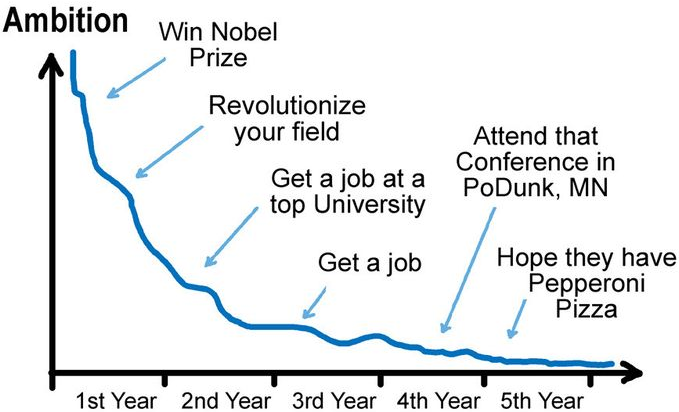
\includegraphics[scale=0.5]{files/c4a.png}
\end{center}

The first two years you typically take coursework (somewhat equivalent to an MS study), find an adviser, and learn how to do research.  The next 2--3 years you focus on your research, form a dissertation topic, and get results published. The last 1--2 years you continue to publish, write and defend your dissertation, and look for a job.
Within these 5--7 years, CS PhD students often take a ``leave of absence'' for 1--2 semesters or summer to do internships at companies and research labs.

The PhDComics figure above shows the ``ambition'' level of a PhD student over their years of study (they miss the 6--7th year when the ambition is \emph{``Just let me graduate''}).

\begin{commentbox}[Vu:]
    I start my PhD with an MS, and it took me 7 years (Fall'07-- Fall'14). I spent half a year doing an internship at the Naval Research Lab. My PhD did take a bit longer than usual, but allows me to explore various research areas and topics.
  \end{commentbox}

\section{My undergrad was not in CS or related areas}\label{sec:non-stem}
\sectioninfo{You can successfully apply to CS PhD even if you have non-CS background.}

You still can apply to PhD in CS \emph{as long as} you can demonstrate you are ready for it through your background, research experience, LoRs, statements, etc. You might be even able to leverage this to make your profile stand out as mentioned in \autoref{sec:improve-your-chance}.

A main question adcom has for a non-CS or non-STEM student is if you have the sufficient technical background obtained through core CS courses.  So you need to show that you have such knowledge through your coursework, projects, or research.
For example, if you have taken a course on Algorithms, even online ones like Coursera, you can talk about it in your SOP.  If you have done a project that requires knowledge of OS or have a professional certification (e.g., A+) through work, you can talk about it.  If you have done research that requires knowledge of Discrete Maths, you can talk about it.  You can also ask your LoR writers to talk about your technical background.
In summary, in your application, convince us that you have the background to do CS PhD research.


\paragraph{Core CS topics} Common CS knowledge that you should know are:
\begin{itemize}
  \item Programming Foundation (e.g., programming concepts in some modern languages)
  \item Discrete Math (e.g., logic, set theory, proof techniques)
  \item Data Structures and Algorithms (e.g., linked lists, trees, sorting, searching)
  \item Computer OS or Systems (e.g., memory management, file systems, processes)
\end{itemize}

In short, you \emph{do not need} to formally take CS courses, you just need to show that you have this essential knowledge, e.g., through the mentioned ways. Many universities are well aware that incoming graduate students might not have all the technical background, so they often have a \emph{``bridge''} courses to help students catch up.  For example, Mason has four bridge courses corresponding to the four core areas above that incoming students can take to catch up on their CS knowledge.


\begin{commentbox}[Vu:]
  I would advocate for a non-STEM student who shows that they have a strong drive for CS by studying core CS knowledge through various channels (e.g., self-study through online courses, projects, etc.).  I have seen many students with non-CS backgrounds who are very successful in CS PhD.  I also have seen many students with CS background who are not successful in CS PhD.  So it is not about your background, it is about your drive and passion for CS research.
\end{commentbox}






\section{Is an MS required for admission to PhD in CS?}\label{sec:msrequirement}
\sectioninfo{You do not need an MS to do PhD in CS.}

No. In fact, students can get MS degree ``along the way'' to PhD, e.g., after finishing the 2-year course work.  However, MS can help admission if it gives research experience or is from a more well-known school than your undergrad institution (\autoref{sec:your-school}).

If you have an MS then some course work \emph{might be} transferred for course credits, which \emph{might} save some time. But in general don't count finishing earlier just because you have an MS. 

\begin{commentbox}[Vu:]
    I start my PhD with an MS in CS from a US university.  I found that the MS helped me in gaining research experience, but I still had to retake courses because I did my MS at a different university.  So in the end, I did not save any time because of the MS.
    
    In general, don't worry if you don't have an MS. But also don't feel that you wasted your time if you have an MS, as it can help you in research.
  \end{commentbox}



\section{PhD in the US vs. Other Countries}\label{sec:non-us-differences}
\sectioninfo{Among several differences, CS PhD in the US does not require an MS degree but has a longer PhD study time.}

\begin{table}
\caption{Comparison of US and Other PhD Programs}\label{tab:us-vs-other}
\begin{tabular}{c|c|c}
\toprule
\textbf{Aspect} & \textbf{US PhD Programs} & \textbf{Other Countries} \\
\midrule
Duration & 5-7 years & 3-5 years \\
MS Required & Not required & Often required \\
Coursework Required & Yes (first 2 years) & No \\
Research Proposal Required & No & Yes (in some countries) \\
Academic (Faculty) Job & Direct & Postdoc \\
Work Life Balance & Less & More \\
\bottomrule
\end{tabular}
\end{table}


\autoref{tab:us-vs-other} summarizes the main differences between CS PhD in the US and other countries. % This is based on my experience and what I heard from others who did PhD in other countries.

\emph{MS requirement and PhD duration}:  CS PhD programs in the US do not require an MS degree (as mentioned in \autoref{sec:msrequirement} and \autoref{sec:time}).  In contrast, many other countries require having an MS degree before joining a PhD program.  This means that US PhD programs are longer (5--7 years, 2 of which are coursework) than other countries (3--4 years, no coursework).

\emph{Project proposal}: in many countries, you have to choose a project and adviser \emph{during} the application process (e.g., you write a proposal to a potential adviser). But this allows you to start your research right from the beginning. 

In the US, you often start your PhD without an adviser or project and find them later. You will have two initial years to explore and find an adviser and research topic. After that you explore projects with that adviser before settling on one (can take a couple of years). 

\emph{Course work}: as mentioned above in the US you will spend the first couple of years taking classes and exploring potential adviser and research topics. 
After that, you have to pass a series of exams during your PhD, e.g., qualifying exam, comprehensive exam, thesis proposal defense\footnote{The word ``ABD'' (all but dissertation) is used in the US to refer to a PhD candidate who has finished all course work and exams and only needs to write and defend their dissertation.}.

In other countries, you start your research right away, e.g., you immediately work on the research project you proposed with the adviser you chose. Moreover, you might not have exams like those in the US or only have to do a few of them.

\emph{Funding}:  In many countries, funding comes from the university or the gov't. This funding often has a fixed duration (e.g., 3 or 4 years).  In the US (\autoref{sec:funding}), funding (e.g., RA) comes directly from your adviser (no fixed duration).  There are also fewer TA opportunities in European universities compared to the US.

\emph{Academic position after PhD}: In other countries, PhD graduates interested in academia typically apply for additional research appointments, i.e., postdocs, and then consider faculty positions. 

In the US, PhD graduates often apply directly for faculty positions. Postdoc for US graduates is no longer a popular option as it was before.

\emph{Work-life balance}: PhD students in the US are often said to be overworked compared to other countries, e.g., in Europe.  This is partly due to the longer PhD program and that US PhD students are often paid through TA, which requires them to do TA in addition to their own research. In contrast, PhD students in other countries are often paid through fellowships, which might not require doing TA.


%% Vu: *what's a PhD?*  This [[https://matt.might.net/articles/phd-school-in-pictures/][series of pictures]] from [[https://matt.might.net][Matt Might]] illustrates what a PhD means.
%% \end{commentbox}


% \section{Timeline}

% \begin{table}[h!]
% \centering
% \begin{tabular}{l|l}
%     \toprule
% \textbf{Month} & \textbf{Task} \\
% \midrule
% January-March & Research programs and prepare for tests \\
% April-June & Take standardized tests (GRE, TOEFL, etc.) \\
% July-September & Prepare application materials (SOP, LORs, etc.) \\
% October-December & Submit applications \\
% January-March & Interviews and follow-ups \\
% April & Admission decisions \\
% \bottomrule
% \end{tabular}
% \caption{Application Timeline}
% \end{table}
% \section{Why the US and not other countries?}
% TODO

\chapter{How is Your Application Evaluated?}\label{sec:evalapps}

\sectioninfo{Applications are evaluated by the \emph{PhD Admission} (adcom) committee and each application is typically reviewed by three faculty members.}

\epigraph{How is education supposed to make me feel smarter? Besides, every time I learn something new, it pushes some of the old stuff out of my brain. Remember when I took that home wine making course, and I forgot how to drive?}{\textsc{The Simpsons}}

After you submit your PhD application, it will first be checked for general requirements, e.g., did you submit your transcripts and standard scores? did your reference writers submit their letters? Usually, this screening process is done through a central university system, i.e., not by CS faculty.

After screening, your application is complete and forwarded to the CS department for further evaluation. If you don't pass screening,  the system will tell you what is missing and what you need to do. So pay attention to your email and check your application status regularly.

\begin{commentbox}[Hakan:]
  At Mason, for full consideration, students should make sure to submit \textbf{ALL} required documents by the application deadline, and should never assume that some required documents (such as official TOEFL scores or official diplomas/transcripts) will be waived by the admissions office. If something is listed and not marked as ``optional'', it is mandatory and they should plan for submitting all those.
\end{commentbox}

\section{Admission Committee (adcom)}\label{sec:adcom}

Your applications are reviewed by a PhD admission committee or \emph{adcom} that consists of faculty members in CS\footnote{In some cases the committee can involve affiliated faculty from different disciplines.}. These adcom members have a wide range of expertise and background to ensure diverse perspectives in the evaluation process. The size and the review load of the adcom depend on the department size. At Mason, the PhD adcom typically has 15--20 faculty, and each committee member is assigned to review about 30 applications. Note that most large schools, including Mason, have separate adcoms for MS programs (\autoref{chap:ms}).

Each application is assigned to about three adcom members, who will evaluate your profile and reach a consensus.  While the assigned reviewers are the main ones deciding your application, other faculty in the department can also have access to your application and provide inputs and opinions on your profile.

The PhD adcom typically involves assistant professors in the department (see \autoref{sec:faculty-types} for various types of faculty). This provides junior faculty the opportunities to recruit students. The chair of the committee will likely be a senior faculty, but they will not review individual applications and instead assign them to committee members. The chair will look at various factors such as research interests or mentioning faculty names to assign the applications to appropriate faculty, e.g., I am often assigned to review applicants interested in software engineering.

\begin{commentbox}{Vu:}
At Mason, we usually decide that a full-time PhD candidate is either (i) admitted with funding (\autoref{sec:funding}) or (ii) rejected. In other words, in most cases, we either
admit you with full funding or reject your application. In some rare cases, we admit
without funding because you have funding on your own, e.g.,
supported by your government or having external fellowships. We justify
our decision (\autoref{sec:ievaluate}) with a summary of your application, where we list
strengths, e.g., a well-known school, and weaknesses, e.g., weak
LORs.
\end{commentbox}

% \didi{Is there more information on typical strengths and common weaknesses of applications. This is especially useful to sophomore and junior students as they still have time to work on those strengths.}
% tvn: the main thing is research experiences


\section{How are decisions made?}\label{sec:how-decisions}
\sectioninfo{Even if all adcom reviewers recommend acceptance, the application can still be rejected. Vice versa, if all reviewers think the application is weak, the student might still be admitted.}

After reviewers have evaluated an application, adcom chair will review all evaluations, look at entered notes, and ask reviewers to discuss and resolve discrepancies to reach a consensus (e.g., a reviewer wants to accept but the other wants to reject).  Typically, the decision is made entirely by the reviewers; there is no involvement from the adcom chair, department chair, or others. In most cases adcom members, even those reviewing the same application, make decisions independently and do not talk to each other (just a common practice to avoid biasing). In some rare cases we might (\autoref{sec:adcom-discuss}).


Even if \emph{all} reviewers recommend acceptance, the application is not automatically accepted, especially if no faculty is willing to advise the student. For example, if the student is interested in a research area that no faculty is working on, or an area where no faculty is taking new students (e.g., AI/ML where faculty likely already has many students) then the student will not be admitted.  This is increasingly common as the number of applicants increases significantly in recent years in CS.

However, if the student has contacted a faculty member and that faculty member is interested in the student and has made this known to the admission committee, then the student is likely to be admitted, \emph{even if the faculty does not review the application or has funding} (thus the importance of contacting faculty). 
Similarly, if the student mentioned a faculty member in their SOP, adcom might ask that faculty member to look at their application and if they are interested in the student.  Even if the student has a weak profile (but still passes the minimum requirement from the university), they might be admitted if a faculty member is willing to take them. Adcom members, especially in the US, are very reluctant to go against the faculty's decision (e.g., if a faculty wants to admit a student, we are not going to reject them).


\section{Do adcom members talk to each other?}\label{sec:adcom-discuss}
\sectioninfo{Sometimes adcom members discuss applicants, but in most cases they make independent decisions.}

However, in some rare cases we do talk to each other.  For example, when there are discrepancies in evaluations, in which case the adcom chair will ask reviewers to discuss the application to reach a consensus.  We also talk to each other for interesting or strong applications, e.g., how to recruit this student or who should be the adviser. 
If the student mentioned a faculty member in their SOP, we might ask that faculty member if they are interested in the student. 



\section{How applications are assigned to adcom members?}\label{sec:applications-assigned}
\sectioninfo{Adcom members only review applications assigned to them (typically matching their expertise) and rarely get involved in other applications}


While adcom members (in fact, any faculty) can view any application, we only review those that are assigned to us, which are already too many. Adcom chair will assign applications to reviewers based on their expertise (e.g., if a student says they want to do SE or interested in working with me), and reviewers will only review those applications. Occasionally we might look at other applications, e.g., if we know the student or have some special circumstances (e.g., if that student contacted me, I know that student, they are from Vietnam, etc). However, even if we look at them, we usually do not get involved in their evaluation.

\subsection{Why CS depts do not waive the application fee?}  

Some universities do waive, e.g., Rice does for all PhD applicants and many universities for domestic students (\autoref{sec:domestic-students}), however most do not for international students.
Some require proof of financial difficulties, e.g., a statement from a financial adviser or a bank statement.

In gneral, application fee is typically a requirement of the university. Individual departments and programs do not have the flexibility to waive the application fee, even if they want to.

\begin{commentbox}{Vu:}
In my opinion, requiring applicants to pay the fee helps ensure their seriousness, as it filters out non-serious candidates. Most CS programs already receive many applications and would be overwhelmed if the application process were free.  Even with application fee the competition is already very tough, imagine if the application is free and the number of applications doubles or triples.\\

Note that if you have financial difficulties, you can ask the department for a waiver, but this is typically only granted in exceptional cases.
\end{commentbox}



\chapter{Your Application}\label{sec:application}

\chapterinfo{The committee will look at various factors, but the most important ones are letters of recommendation (LORs),  statements of purpose (SOP), and research experience and potential, e.g., publications.}

\epigraph{Son, if you really want something in this life, you have to work for it. Now quiet! They’re about to announce the lottery numbers.}{\textsc{The Simpsons}}


The goal of adcom is to evaluate your research experience, potential, and interest to see if you \textbf{fit into our PhD program}! The emphasis here is \emph{fitting}, which varies from school to school, faculty to faculty, and even from year to year.  However, in general, to evaluate your profile, we consider the following key indicators.


\section{Letters of Recommendation (LOR)}\label{sec:lor}
\sectioninfo{\emph{LORs are very important}, but only if they are personalized and talk about your research ability.}

\begin{center}
  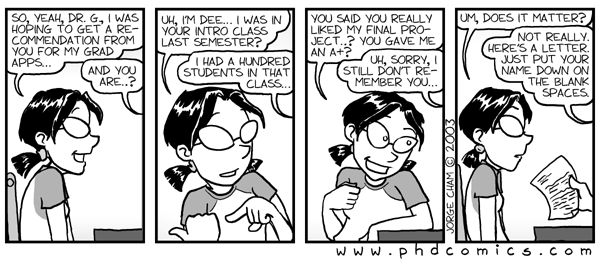
\includegraphics[width=0.6\linewidth]{files/c6.png}
\end{center}


Most PhD programs will require at least \textbf{two LORs}. 
The goal of the LoR is to provide the adcom with an assessment of your research ability and potential. 
The letter should 
focus on your research background, achievements, and potentials, all of which paint a compelling picture of the candidate to the adcom.

\paragraph{LoR writers} LoR writers should be someone who (i) can talk in depth about your research experience and potential and (ii) have the credibility to evaluate your research ability.  

A LoR writer should be someone who knows you well, so that they can provide a strong-supporting and personalized letter for you.  
LoR writers should also have the credibility to convince adcom members. Such a person is typically someone who has a PhD (so they know what a PhD is about) and is active in research (so they can evaluate your research ability).
LoR writers are often your research advisers, professors, or supervisors who have worked with you on research projects.


\paragraph{LoR from Famous People} Having a strong letter from an internationally recognized researcher will \emph{greatly strengthen} your application. A strong LOR from such a researcher can outweigh the lack of publications (or low GPA or unknown school).

%However, obtaining letters from famous people
%can be challenging for international students, who might not have many interactions with such experts.

However, let's face it.  Most of us don't have an opportunity to interact or work with well-known researchers.  
So what to do? It is perfectly fine to have a letter from people who know you well enough to talk about \emph{your research experience and capabilities}. These include profs., researchers, postdocs who have mentored and worked with you. In fact, a personal, customized, and strong letter from even a senior PhD grad student who mentors and knows you well is much better than a generic letter from a well-known superstar who does not know you well. 

It is also worth noting that a LoR from a ``full'' senior professor who has not been active in research might not be as strong as a LoR from a junior faculty who has been actively mentoring you in research.  This applies to administrative (e.g., chairs, directors, and deans) also (\autoref{sec:admin-letters}.) The fame of the writer is less important than how well they know you and can write about your research ability.

Many students get letters from supervisors from companies where they did internships or are working.  It is OK as long as it is a research-based personalized letter. Again, the emphasis here is \emph{research}, i.e., the letters should describe your research experiences and potential. Letters focusing on your coursework or non-research projects at a company won't carry much weight.

\begin{commentbox}[Vu:]
  If your grading system is not US standard, or you are from a good school unknown outside your country, you can ask your reference writers to explain that in their letters.  For example, ``Bach Khoa'' are the top universities in Vietnam for STEM studies but few people outside Vietnam know about them.  So if you are from there, you should ask your reference writers to mention that.
\end{commentbox}


\subsection{Generic Letters are Bad}\label{sec:generic-letters} 
When the writers do not know much about the applicants (e.g., just taking some course with them or not making any impression to write about), they might write a generic and short letter, which is not useful and also considered weak. 

This does not mean the professor is not good or does not care about you, but they just do not know you well enough to write a strong letter.
So it might be a good idea to directly ask if the prof. is willing to write a \emph{strong} letter for you. If not, then you should ask someone else.  For example, if a student I don't know well asks me to write a letter for them, I will explicitly tell them I don't know them that well to write much about them, and such a short, generic, and weak letter will not help their case.


\begin{commentbox}[Hung:]
  A sad reality is that most professors in Vietnam \textbf{DO NOT} know how to write a good letter, or are lazy in writing letters hence delegate the writing to the students. Unfortunately, there is no easy solution to this problem.
\end{commentbox}

\begin{commentbox}[Vu:]

  Several international students mentioned that some professors are unwilling to write letters or write weak ones because they do not want (good) students to go abroad or only go to places where they want the students to go to. If you are in this situation, you should find someone else to write for you.
  \tcblower

Sometimes students would go to great lengths just to get letters from well-known professors in their school (e.g., department head or dean). But as mentioned, if these professors do not know you, their letters would likely be generic and carry little value (sometimes \red{red flags}). Moreover, a top professor at your university might not be well-known to US faculty (see more details in \autoref{sec:admin-letters} and \autoref{sec:your-school}). So save the trouble and get letters from \emph{any} professors/supervisors who know you well and can write a good letter about \emph{your} research ability. It's better to have a good personalized letter about your own research ability from someone who is less well-known than a generic/weak letter from a well-known person.

\end{commentbox}


\subsection{Self-written Letters are Bad}\label{sec:self-letters}
 Many international students write letters themselves, typically due to the requests of their profs. or letter writers. Such letters have \emph{little value} and are considered weak by reviewers---why can you not even find someone who cares or knows enough about you to write a candid personal reference letter?  Instead of the ref. writer talking about you, in this case it is you who write about yourself (and they just sign the letter). Experienced reviewers can easily spot  (because the student often has little experience in writing LoRs) and  \red{red flag} such letters.

\begin{commentbox}[Vu:]
 Well-known and well-respected profs would \emph{not} ask you to write your own letter (in fact, even not well-known ones wouldn't do this to students they care about). This might be a common practice at specific universities and the students do not have a choice as they need the letter.  However, think about this: if a prof. does this often, then they either don't know how to write a LOR (more common than you would think) or simply do not know or care enough about you.  In any case, such LoRs are not useful and might even hurt your application.  So if you are in this situation, you should find someone else to write for you.
\end{commentbox}

\subsection{LoRs from Admin People}\label{sec:admin-letters}

Many international students try to get LoRs from high-ranking administrators in their universities such as department chair/head, dean, or director. The students never worked with these people (they might take a class or so with these profs), but mistakenly believe that these LoRs are valuable due to the writer's high position in the university.
However, as emphasized, a generic LoR has little value because the writer does not know you well and can talk in depth about your research ability. 

Moreover, while being well-known and respected in your local university, these writers might not be very active in research (e.g., they haven't published in recent years). Thus they might not be well-known and recognized by adcom members.  

\begin{commentbox}[Vu:]
  In my experience in reviewing applications, letters from admin people are often generic and do not provide much value. 
  In many case, the letter reads like it was written by a student (\autoref{sec:self-letters}), and thus is a red flag.  So if you are in this situation, you should find someone else to write for you as mentioned in this section.
\end{commentbox}



\subsection{Waiving Your Right}\label{sec:waive-right}

When you ask someone to write a letter for you, you will be asked if you want to waive your right to see the letter.  You should \emph{always} waive your right.

Choosing not to look at a reference letter is pretty standard in school and job applications. When you waive your right to see the letter, it adds a layer of trust, showing you're confident in your choice of referees and that you're not trying to twist their words. It's also about keeping things open and honest between you and your letter writers and encourages them to be real about your strengths and qualifications. Plus, it keeps things private.

If you do not waive your right,  the letter writer might refuse to write for you or write a generic letter that does not help your case.  Reviewers also might raise concerns about a letter that is not waived, e.g., if you do not trust your letter writers, then you should find someone else to write for you. In short, it's a standard practice and a way of keeping things straightforward and respectful in the whole recommendation game.

\begin{commentbox}[Didier]
  \emph{Should letter writers have PhDs?}  In Rwanda, a lot of students interact more with teaching faculty who might not have PhD.
  \tcblower
  \textbf{Vu}: This is an interesting and useful detail that US faculty might not be aware of. Students should mention this in their statements. In general, someone with a PhD has been through the research process and therefore can better evaluate your research ability.  But if you do not have such people, then someone who can properly evaluate your research ability is still OK (and again, explain that in your SOP).
\end{commentbox}


\subsection{Help your LOR Writer}\label{sec:help-your-LOR-writers}

As mentioned above in \autoref{sec:self-letters} and \autoref{sec:generic-letters}, do not write your own letter and generic letters do not give much value. Thus, to help your writer to write a strong, customized LoR, you should provide them details or unique things about yourself. For example, let them know about your GPA, research and work experience, papers (if any), or anything you want them to mention.  If the GPA in your program is highly competitive (\autoref{sec:gpa}) and they know that, remind them to talk about it in the LOR. 
You can also provide them with a draft of your SOP so that they can see what you are saying about yourself and complement that with their own perspective.

Sometimes your writer will explicitly ask you for such information, but if not, you should provide it anyway (especially if you have not interacted with them much or have not done much research with them).


\subsection{Remind Your Writers}\label{sec:remind-writers} 

After you submit your application, you should tell your writers about that and let them know they will soon receive an email from the university to submit their letters.  You should also remind them when you submit your application and ask them to submit their letters on time if they haven't done so.  Note that most places only have deadlines for the applicant, but are very flexible with the letter writers (in many cases do not even give them any deadline).  Also, many places do not begin the admission review process right after the deadline and work on application reviews in the next semester (mid-January).  

Thus you do want to send reminders because professors can be quite busy and might forget to submit their letters, especially when there is no explicit deadline. However, do not send too many reminders as that can be annoying to the writers.


\subsection{Thank Your Writers}\label{sec:thank-writers}

After your application is submitted and your writers have submitted their letters (i.e., the wait begins), you should send a quick thank you note, which serves both as an acknowledgement that you know they have submitted the letters and as an appreciate for their help.  You should also let them know the outcome of your application, regardless of whether you are admitted or not.  In addition to being a common courtesy, this can also help maintain a good relationship with your writers, which can be useful in the future (e.g., if you need another letter for another round of applications or for a job reference).


% \begin{commentbox}[Vu:]
% For Vietnamese students, it's worth mentioning the \href{https://vef2.org/}{VEF2.0 program}, which has helped many students gain admission to top CS PhD programs in the US. VEF2.0 invites US faculty members from leading institutions to conduct rigorous interviews with VEF students and subsequently provide reference letters on their behalf. Despite the limited interaction between the interviewer and the interviewee (primarily just the interview), these reference letters are generally effective and have helped many students get into good PhD programs.
% \end{commentbox}


\subsection{How do you write LoR? Is it lots of work?}\label{sec:lor-writing}

If a student asks me to write letter for them, I will agree as I believe it is part of my job. However, I will ask them to waive their right to see the letter (\autoref{sec:waive-right}), and will not write if they do not do so.

I will also let the student know if I can write a strong letter for them.  If I can't, I will tell them and suggest they find someone else.  If they insist, then I will write for them. While I try to say something positive, e.g., the student is hardworking, or that I heard they are working on a research project, etc, the letter will still be short and weak (\autoref{sec:generic-letters}). Usually it takes me about 5--10 minutes to write such a letter.

For students who I know well, i.e., strong letters, then writing will take a lot longer as it will be personalized.  While I have a general template of such strong letters, it still can take me an hour or more to write such a letter.  I often ask the students to provide information (\autoref{sec:help-your-LOR-writers}) and what they think I should highlight in the letter. They can also provide me their SOP (if they already have written one) so I can complement what they say with my own perspective.


%\subsection{Will it annoy them if they have to submit many letters? }\label{sec:many-letters}
%Profs. are used to write letters for their students


\section{Statement of Purpose (SOP)}\label{sec:sop}
\sectioninfo{\emph{SOP is important}. Write it in such a way that makes you \emph{stand out}.}

\begin{center}
  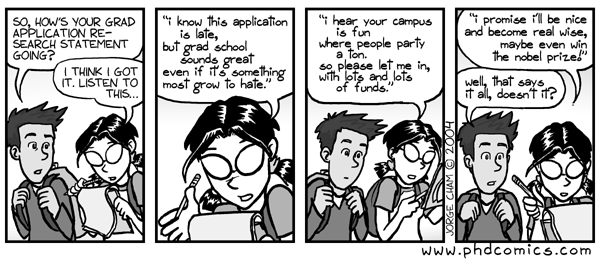
\includegraphics[scale=0.5]{files/c2.png}
\end{center}

While you might not have control over LORs (\autoref{sec:lor}) or where your go to school (\autoref{sec:your-school}), you do over your
statement of purpose (SOP) or personal statement\footnote{Few schools separate these documents and ask you to write both: SOP, which focuses on research experiences, and personal statement, which is everything more personal, e.g., why PhD, challenges, diversity, etc}! A well-written SOP also shows that you can communicate, which is very important in research, and that you can effectively teach and communicate with students, which is important for TA funding (see \autoref{sec:funding}).  Many SOP samples for CS are \href{https://cs-sop.org/}{available here}.  

%In your statement, you have the opportunity to connect directly with adcom members and make your application stand out and unique. Your SOP can convince adcom members that you would \emph{fit} their program, even if you don't have very strong research experience.
% is important because if you need (GTA) funding, it will provide evidence
% that you can teach and communicate with students.

In your SOP, focus on research potential and convince us through your experience, e.g., published papers. Back up your claims with \textbf{concrete evidence}. For example, if you say you have experience with teaching, then show what you did, e.g., undergrad TA or mentoring someone.  If you say you work on a project, then show some results, e.g., paper submitted (or even rejected), achieved certain performance improvement over the state of the art. 


You should talk about things that adcom members might not know about and can help make you \textbf{stand out} in the application pool of thousands of applicants, e.g., you are member of a minority or LGBTQ+ group (\autoref{sec:urm}), your personal Github project with hundreds of stars or your regular contributions to well-known open-source projects (see \autoref{sec:improve-your-chance} for increasing your admission chance).


This is a simple task often overlooked by many applicants: \textbf{tailor your SOP} to the institution you're applying for,
e.g., why do you apply \emph{here}? who do you want to work with?
Provide names of professors who you're interested in (if they are not already in the adcom, your application might get forwarded to them for evaluation; and they might be interested in interviewing and recruiting you).
This shows that you're serious and have done homework on places you're applying to.
Adcom will look for this part (\autoref{sec:why-rejected}).

Finally, your SOP reviewed by your LoR writers and professors, especially those who have served in adcom, or even postdocs or PhD students as they have been through this process.

\begin{commentbox}[Vu:]
  I often read LORs and SOP first (\autoref{sec:ievaluate}). If I am
  persuaded by then, I would skim over other factors and advocate for
  admission (unless I see red flags in other parts). However, if I am not
  convinced, then I will likely recommend rejection (unless I see
  something stand out in other parts).
  \tcblower
  Do careful research on professors, don't mention \emph{emeritus} or adjunct faculty (see more about various types of faculty in \autoref{sec:faculty-types}).
  Also, be careful not to send statements to the wrong schools or mix
  facts (e.g., talking about school X but mentioning working with
  profs. at school Y; and do not talk about George Washington when applying to George Mason). I have seen such statements more times than I should.
\end{commentbox}


\subsection{Kiss of Death in SOP} \label{sec:kiss-of-death-sop}

\begin{itemize}
\item \textbf{Too personal} Don't talk about your personal issues, e.g., family, health, relationship, etc. This can raise concerns about your ability to handle the PhD. Don't talk about religious or political beliefs (\autoref{sec:cultural}).
\item \textbf{Criticizing} your current or previous institution or professors: just like in a job interview, don't badmouth your current or previous employer. 
\item \textbf{No concrete evidence to back up claims}: e.g., saying you are passionate about a research topic without showing any experience. This is where specific names (work submitted at conf. X), numbers (outperformed SOTA by Y \%), and examples (worked on project Z) can help. 
\item \textbf{Use flowery and AI-like language}: don't use AI to write your SOP. Not that hard to raise suspicion.
\item \textbf{Not customized to the program}: If your SOP can be sent to multiple programs with few changes, it is too generic. Do some homework and mention why you want to spend the next 5--7 years there.
\item \textbf{Mentioning wrong professors}: do not mention emeritus professors or those who have left.  Do your homework to see if the professors you mention are still active in research.  Teaching and adjunct faculty are often not active in mentoring PhD students (\autoref{sec:faculty-types}).
\item \textbf{Too Long and fancy format}: As mentioned, keep it under 2 pages. Don't use too much coloring or fancy fonts (like those in Words). CS academics like using LaTeX (common way to write our papers and other documents), so write your SOP using LaTeX. 
\end{itemize}


\subsection*{Additional Resources}
\begin{itemize}
    \item \href{https://chrisblattman.com/blog/2022/01/11/}{Writing your statement of purpose} by Chris Blattman
  \item \href{http://www.pl-enthusiast.net/2022/10/03/how-to-write-a-grad-school-personal-statement/}{How to Write a Grad School Personal Statement} by Mike Hicks
  \item     \href{https://cs-sop.notion.site/cs-sop/CS-PhD-Statements-of-Purpose-df39955313834889b7ac5411c37b958d?p=f5d5980a71524ebaa4e6ae57266b847c&pm=s}{CS PhD SOP database} by cs-sop.org
\end{itemize}
% \subsection{Outline of a LOR}\label{sec:lor-outline}


\section{Research Experience}\label{sec:research-experience}

\sectioninfo{\emph{Publications can greatly help}. Papers in good venues are concrete evidence that you have successfully engaged in research. But they are not required!}

This section discusses publications and other research experiences that can strengthen your application.
\autoref{sec:research-opportunities} provides more information on how to find research opportunities (e.g., during your undergrad study).

\subsection{Publications} The most concrete evidence of research ability is having \emph{papers in reputable international journals or conferences}.
Having published papers, especially at top venues, is a sign that you have been successfully involved in research. 

Publications are never required for application, however given the competitiveness of CS admission, they can significantly strengthen your application and are becoming the norm. Applicants admitted to top schools, especially in popular fields such as ML and NLP, often have multiple first-authored papers at top places.

\begin{commentbox}[Vu:]
  Many international students mention Scopus Q1, which consists of various journals from IEEE, Elsevier, and many other publishers.  I don't know/recognize many of the journals listed in Scopus Q1. This might be something to be mindful of, as \textbf{CS} faculty might not be too familiar with Scopus or journals listed there, so devote some part in your statement to discuss the significance of your papers.
\end{commentbox}

\begin{commentbox}[Thanh:]
    Due to academic culture, professors in Vietnam usually aim for (international) journals instead of conferences. Could you give some tips on how to know whether a journal is good (CSrankings, unfortunately, only consider conferences)?
    \tcblower
    \textbf{Vu}: One way is looking at what well-known researchers publish. For example, if you are interested in a field X, you can use CSRankings to look at active faculty in X, and then look at their websites to see what journals they publish at.
\end{commentbox}
\paragraph{What if I don't have any pubs} It is understandable that many students do not have the opportunity to publish papers. Thus, other writings, even those under submissions or rejected, would still be good and better than nothing.  Be sure to upload your papers with your application and talk about them in your statement (see \autoref{sec:sop}).  

Note that local conferences and non-English journals or conferences do
not carry as much weight since their quality is often unknown to US faculty. However, if you have published in such places, you should still upload them, mention them in your statement, and explain why they are good.

% In CS, conferences are important and top conferences are prestigious. You can find top CS conferences at places such as \href{https://csrankings.org}{CSRankings}, which ranks CS programs based on how their faculty publish at top \emph{conferences} (see more in \autoref{sec:ranking}).

\paragraph{I am not the first author} Being the first author is good because it indicates you own the work. However, it's perfectly OK to be second or third or last.  It is difficult to publish a good paper and so being a co-author is still a good sign about your research experience. In any case (and especially in the case when you're not the first author), you should explain the work and your contribution.  Better yet, have your LoR writers talk about your contribution in their letters.

\begin{commentbox}[Craig:]
  Mason and many other universities allow you to upload your published papers and other writing samples. In many cases, even if the papers were not published at top places, we can still determine their quality by simply skimming over the paper.
\end{commentbox}



\subsection{Work Experience} Work experience at \emph{well-known research laboratories}, such as Microsoft Research, can strengthen your
application.  Unfortunately, many good research places in your countries, e.g., VinAI in Vietnam, remain relatively unknown to most universities in the US. So you or your LoR writers should explicitly say something about them in your statement.  In general, if you did some good research work at such places, then you should mention that in your SOP and ask your supervisor to write about your research experiences and potential in their LORs (\autoref{sec:lor}).


\begin{commentbox}[Hung:]
  The reputation of VinAI has been increasing steadily over the past few years; many of my colleagues heard about VinAI.
\end{commentbox}

On the other hand, if non-research work (e.g., software development) \emph{do not} carry much weight for PhD (they can help for MS application though). Similarly, LoR from your supervisor for non-research experience will not count much.
So do not spend much time talking about non-research-related job in your SOP.



\subsection{Competitions} Winning \emph{internationally recognized competitions} can demonstrate your research potential.
For example, participating in Math Olympiads if you want to do theory or winning ACM programming contests if you want to ``build'' systems, e.g., software analysis.




\section{Your School and Grades}\label{sec:your-school}
\sectioninfo{\emph{High grades probably won't help much} (unless you're from a very top and well-known school), but bad ones likely will raise concerns.}

\subsection{School} Graduating from top universities \emph{that we recognize} helps. For example, if you are an international student and your school is well-known, then it is \emph{``top foreign''}, which is a plus.
However, if we do not know much about schools in your country, then we are uncertain about the quality of your school and likely treat your school as \emph{``unknown foreign''}, which can be a minus point.


Many international students mistakenly believe that their school is well-known, but in fact, it is not (e.g., many Vietnamese students believe that ``Bach Khoa'' is well-known internationally, but it is not).  So you should explicitly mention that in your SOP and ask your LOR writers to do that as well. 
Of course, if you're interested in working with Vietnamese, consider  \href{https://github.com/dynaroars/dynaroars.github.io/wiki/Viet-CS-Profs-US}{CS programs in the US that have Vietnamese professors}. %It might also be helpful to have your CS dept to put itself on CSRankings so that others know about the dept, its faculty, and research.

\begin{commentbox}[Vu:]
  Sometimes PhD adcom in the US will share a document such as \href{https://github.com/dynaroars/dynaroars.github.io/wiki/Foreign-Top-Schools}{this one}, which lists the top schools in several countries. We also ask other faculty and students if we think they know about the place.  For example, when I was a postdoc at UMD, members of their CS PhD adcom asked me to evaluate applicants from Vietnam.  During my time at UNL and now here at Mason, I have looked at Vietnamese applications (whether they are assigned to me or not) and provided input to their reviewers, e.g., X is the top tech school in Vietnam and so it should be \emph{top} instead of \emph{unknown} foreign, which makes a huge difference.
\end{commentbox}
\begin{commentbox}[Deepak:]
  If an applicant is anxious about their school not being known outside their country, they can provide information about their school and department, with independent sources where such information can be verified.
\end{commentbox}
\subsection{Grades}\label{sec:gpa}

Grades generally do not matter much for CS PhD admission. PhD in CS is a research degree and doing well in undergrad courses does not necessarily mean you can do research (other factors such as research experiences, pubs, LoRs are more important).

Nonetheless, if you are from a well-known school, having good grades do help (not a lot though), e.g., adcom members often note details such as "good GPA from well-known school (\autoref{sec:ievaluate}). However if your school is not well-known, having top grades or rankings usually will not help because we cannot evaluate them (e.g., we don't know how hard it is to get a 4.0 or A's at your school). This can be an issue for students in many top international universities where the competition is so high that very good students can still have low rankings from these schools (and be overlooked by adcom).

As with school reputation, you and your LoR writers can mention the grading system of your university if you think that is helpful for adcom to evaluate (\autoref{sec:help-your-LOR-writers}).


\begin{commentbox}[Thanh:]
    Vietnamese universities typically offer specialized programs, such as the talented engineer program at HUST, that have highly competitive entrance exams and a limited number of available slots (e.g., 30 per year). However, these programs often set higher requirements for students, including more demanding tests and assignments, resulting in lower GPAs and overall rankings. For example, 3.5 GPA students from such talented programs are typically much better than 4.0 GPA students not in those programs.  Similarly, variations in GPA standards exist among different universities, with technical universities generally having lower GPAs than economic universities. These make gaining admission in the US difficult as US faculty are not familiar with these issues.
    \tcblower
    \textbf{Vu}: Vietnamese students and even faculty often lament how this grading system hurts Vietnamese students applying abroad. One way to mitigate this is to make these issues known in your SOP.  \href{https://github.com/dynaroars/dynaroars.github.io/wiki/Viet-CS-Profs-US}{Universities with Vietnamese profs} are probably aware of them, but in general your letter writers \emph{and} you can explicitly mention these in their letters and your statement.
  \end{commentbox}

  
\paragraph{Bad Grades} 
While having good GPA might not help much (again, because of other much more important factors),
having bad GPA can hurt your application.  Many universities have a minimum GPA requirement (e.g., $> 3.0$) and will automatically reject applications with lower GPAs.  
If you have bad grades, you should explain them in your SOP or better yet, have your LOR writers explain them in their letters if they know the reasons.

Moreover, having bad grades in relevant courses, e.g., Math and CS, can be a \red{red flag}.
Adcom members often scan through transcripts (\autoref{sec:ievaluate}) looking for C and lower grades in Math and CS courses and might raise concerns if they see several of them.
Note that bad grades in non-relevant courses, e.g., e.g., about politics or history, are not as concerning.

Should you explain bad grades in relevant courses in your SOP?  If you have just a few,  they do not matter much, so don't spend much time explaining them (many adcom reviewers themselves have bad grades in relevant courses!). But if you have many bad grades for an entire semester or year due to some specific reasons, then you should explain them in your SOP.

\section{Standard Tests (e.g., GRE and IELTS), Online Courses, and Certificates}\label{sec:standard-tests}
\sectioninfo{\emph{Standard tests are not important}. GRE typically \emph{is not} required. For standard English tests (not required for domestic students), just do enough to pass the minimum requirements.}

\subsection{GREs Are Optional and Do Not Matter} While a few schools still require taking the GRE (e.g., UCF), most good CS PhD programs in the US \textbf{no longer} require it. Thus, if you haven't taken the GRE or have bad scores, then don't waste time (re)taking it. Being optional really means optional, and not taking it will not hurt your application.

However, if you took it and have really good scores then it might be worth it to include and talk about them in your application, but don't expect them to make much difference (many adcom reviewers never took it). But if your scores are bad, then you should not include them in your application, which can be a \red{red flag}.

\subsection{English Tests (IELTS, TOEFL)} Unless your degrees are from specific countries such as \href{https://github.com/dynaroars/dynaroars.github.io/wiki/About-Mason#standard-tests-waiver-eligible-countries}{these}, you will need to take standardized English tests. On one hand you will need to show some level of English proficiency, but on the other hand, you do not need to have very good scores in these tests (many adcom members themselves were once international students and struggled with English).
You should just do well enough to pass the minimum requirement set by the university. %, which is required for TA (\autoref{sec:funding}).
Just as with grades (\autoref{sec:your-school}) and GRE, having high scores in these tests might not help, but having too low scores can be a \red{red flag} and sometimes results in an automatic rejection (\autoref{sec:why-rejected}), e.g., below the minimum requirement.


\begin{commentbox}[Vu:]
  Here is the minimum requirements at Mason. 
  Being above this might not mean much, but below is a \red{red flag}.
  \begin{itemize}
    \item GPA: $\ge 3.0$ in your undergrad (but we also consider the rank/prestige of your school)
    \item GRE: not required 
    % \item but if you want to use it, then we expect a total (V+Q) of $\ge 311$ (with a $\ge 157$ Q) and A $\ge 3.0-3.5$.
    \item \href{https://www.gmu.edu/international/english-language-requirements}{English proficiency requirements} (one of the below)
          \begin{itemize}
            \item TOEFL: 80 OR
            \item IELTS: $\ge 6.5$ OR
            \item DuoLingo Graduate English: $\ge 120$ OR
            \item Pearson Test of Academic English: $\ge 67$
          \end{itemize}
  \end{itemize}
\end{commentbox}


\subsection{Online Courses and Certificates}

These do not carry much weight as they do not show research ability. We do not care much if you have taken an online Coursera AI course or have a professional certificate from Microsoft.
However, as mentioned in \autoref{sec:non-stem}, if you do not have a CS background, you might be able to use these to show you have sufficient CS knowledge.

\section{CV/Resume}
\sectioninfo{Highlight and summarize major achievements, e.g., Publications, Programming Awards}

The CV/Resume provides a summary of the applicant's achievements. Most schools require you to upload your CV with your application.
Prepare your CV in such a way that it allows the reviewers to quickly scan to identify major achievements, e.g., Publications, Programming Competition Awards, and Teaching Experience.

\begin{commentbox}[Vu:]
    Unlike a job application, CV is not as important for PhD admission. We care more about your LOR, SOP, etc.  So do not spend too much time on your CV, just make sure it is easy to skim through and well-organized around research activities and achievements.
\end{commentbox}
  

\section{Interview and the Waiting Game}\label{sec:interview}
\sectioninfo{Getting an interview is typically a \emph{good sign}; but no interview does not mean rejection}

After you submit your applications, the waiting game begins! For many students, this is a very stressful time. This section provides some information and tips to help you get through this time.

\subsection{Interviews} 

After you apply, you might get interviews. The most common case is that a prof. is interested in working with you and wants to chat with you, e.g., to offer RA (\autoref{sec:ra}). In some cases, the interview is done by several professors, e.g., to see if a student fits in their group or to recruit a very strong student to their program. 

Typically, an interview takes about 15--30 minutes, and one important aspect of evaluation is your ability to effectively communicate, including speaking and understanding English. 
You might be asked to talk about your research experience and interests and to read a paper and discuss it. In some rare cases you might also be asked to solve a problem (one of my colleagues at Mason often does coding interview).
The interview is also a good opportunity for you to ask questions, e.g., about the prof, their group, the CS PhD program, and the university.

You should treat the interview as an informal chat. Have ``elevator pitches'' about your research experience and interests. You might also want to have a 5-minute presentation about your research. If a prof. asks you to read a paper, do it and be prepared to discuss it. You can also ask if you need to prepare for a coding problem. Finally, prepare some thoughtful questions to ask, e.g., about the program, the university, or the professor's research (see \href{https://github.com/dynaroars/dynaroars.github.io/wiki/Answers-to-Ph.D-Advisor-Guide}{some questions} you can ask a potential adviser).

\begin{commentbox}[Vu:]
  At Mason, faculty are encouraged to interview candidates. For very strong candidates, the interview is actually to recruit them.  In some cases a faculty interviews a candidate that they see potential and want to advocate for their admission. Without the interview, such applications may be more likely to be rejected.\\
  
  In short, getting an interview is a good sign; it means that someone is considering you. If we are not interested in your application, we will not proceed with an interview.
\end{commentbox}

\paragraph{Follow-Up Emails} If you had an interview and have not heard back, you can email to ask about the status of your application. See \autoref{sec:accept-postpone-decline} for how to check status and follow-up emails.

\paragraph{When do interviews happen?}

The timeline for interviews varies.  Faculty set up interviews based on their (busy and erratic) schedule. Do not be surprised if you get an interview invitation at the last minute. Some schools do not do interviews at all (\autoref{sec:no-interview}).


\paragraph{Updating your profile} You should not send emails to update your profile.  However, if you have new publications or other big achievements, you can ask them to update your application (though no guarantee that they will consider them).

\subsection{Not Getting Interviews}\label{sec:no-interview}
While it is generally good to get an interview, not getting one \emph{does not} mean you're out.  Many programs do not have the tradition of interviewing applicants. For example, at Mason, most admitted students with TA (\autoref{sec:ta}) do not go through interviews.

However, no interviews mean that you will not likely get an RA (\autoref{sec:ra}), which is offered by an individual faculty (if they want you to do research for them, then they likely will interview you first).  If you have no interviews, your application (and TA/fellowship funding) is decided by the adcom.



\subsection{Notification Timeline: Why rejection letters are sent so late?}\label{sec:late-rejection}
\subsectioninfo{Grad programs often wait for the accepted students to make their decisions, typically by April 15, before sending out rejection letters.}

%"Just reject me already!" is a common sentiment among applicants.  Indeed, school will first send out admission offers to the top candidates. They do not send out rejection letters because there is still a chance that some of the top candidates will decline the offer. If they do, then the school will go to the next set of candidates and send out offers to them.  This process continues until all spots are filled.  This is why you might not hear back until late in the admission cycle.

Some schools send out admission letters in batches, some do rolling admission, and some do not send anything out (e.g., you're on their waitlist). You should hear back from most schools by mid-March (though rejection can come out very late).

Not much you can do other than to be patient and wait. Do not send emails asking about interviews or status (unless you have interviewed specifically with someone (\autoref{sec:interview}) then you can ask that person for status updates and other questions (\autoref{sec:accept-postpone-decline}).



\paragraph{Acceptance Letters} Universities prioritize sending out acceptance letters first. This allows the admitted students to make decisions and plan for their studies.

Some universities have rolling admissions, meaning they send out acceptance letters as they review applications (e.g., some universities sent out letters as soon as early February). Others have a specific date when they send out the first round of acceptance letters.   

\paragraph{Response Deadlines} Accepted students are usually given a deadline to make decisions on their offers, often around \textbf{April 15th} in the US. This is a standard deadline for PhD programs due to the Council of Graduate Schools (CGS) Resolution (\href{https://cgsnet.org/wp-content/uploads/2024/01/CGS_April15_Resolution_Jan312024.pdf}{see more}. After this date, CS programs can gauge how many slots remain unfilled.

\paragraph{Waitlist} Most CS programs have a limited number of slots for PhD students, and thus put many good students on a waitlist.  If accepted students decline the offer, then offers are sent to students on the waitlist. So if you see people getting accepted, that does not mean you are out yet.

\paragraph{Rejection Letters} Schools typically start sending out rejection letters to remaining applicants \emph{after they have finalized their admissions decisions}. Thus, rejection letters are often sent out late (e.g., after April 15th or even much later). Not much you can do here. You can try to contact the school to ask about your status, but they might not reply, they might say they are still reviewing applications, or give you inaccurate information (e.g., you will hear in two weeks). In short, you just have to be patient and wait (and also beware that some schools do not send out rejection letters at all).

% \section{Preparing and Tracking Applications}


% \paragraph{Shared Spreadsheet} Many students use a (shared) spreadsheet, e.g., Google Sheets/Docs, to help them and their letter writers to keep track of their applications. Here are some information to put on the sheet.
% \begin{itemize}
%   \item \textbf{Your info}: Full name, email, phone, link to website/CV.  This is helpful for the writers just in case they want to quickly get some information about you.

%   \item \textbf{Applications details}: University, Dept, Application System URL, Submission Deadlines, Application Status (e.g., submitted,  rejected, wait-listed, accepted)

%   \item \textbf{LoRs}: Writer 1, Writer 2, Writer 3.  If this is a shared document, you might want to omit names and just use writer X. Under each is their status, e.g., sent/not yet/reminder needed, etc.


% \end{itemize}


% You can then share this sheet with your reference writers and remind them to submit LoRs on your behalf (see \autoref{sec:lor}). Also, you should periodically update your writers with your status; a simple note such as \emph{``I am getting interviewed by prof. X at school Y. Do you have any advice?''} can get you a lot of help.


% \paragraph{Communicating with LoR writers and People Who Support You}

% stressfull time, rely on support from others
% ask ppl to review your SOPs
% provide information for LORs, ..
%


\chapter{Getting Admitted}\label{sec:accepted}
\chapterinfo{Congrats! Now it is your turn to evaluate the school!
Attend \emph{Open House} to learn more about the place and \emph{interview} profs---they would be much more willing to talk to you now.}

\epigraph{``Oh... and how is education supposed to make me feel smarter? Besides, every time I learn something new, it pushes some old stuff out of my brain. Remember when I took that home wine-making course and I forgot how to drive?''}{\textsc{The Simpsons}}

By around March you should hear back from most PhD programs that want to admit you. 
But you likely won't hear back from schools that do not want to admit you (\autoref{sec:late-rejection}).

If you receive offers, congratulations!  Now you're at a different game because the schools that have admitted you will try to get you to accept them!  Important factors to consider include the reputation of schools and professors (\autoref{sec:schoolsandprofs}), and funding availability (\autoref{sec:funding}). You will likely have to make your decision (\autoref{sec:accept-postpone-decline}) by around \emph{April 15}, which is the deadline for most schools
(\href{https://cgsnet.org/wp-content/uploads/2024/01/CGS_April15_Resolution_Jan312024.pdf}{why this date?}).

\paragraph{Open House} Most schools have \emph{Open House} or \emph{Visit Day} events, which are a great resource to learn about the school, department, faculty, research, living, etc.

Even if you can't come in person, you should attend virtually and meet with individual faculty. During the event, you get a chance to learn more about the program, and talk to individual faculty and current students.  Take notes of faculty who make you excited, and count those taking in new students (if they meet you, likely they are considering new students!).  Talk to students about their advisers, the dept, the area, and the funding situation.  Ask about anything you want to determine that they deserve \emph{you}.

\begin{commentbox}[Vu:]
  Mason has \emph{Virtual} Open House (VOH), e.g., \url{https://cs-Mason.github.io/cs-phd-voh-s23/}. We invite all admitted PhD students to the VOH through Zoom to learn about the CS program, the department, Mason, and the DC area in general. Students also get opportunities to chat with professors and current students.
\end{commentbox}

\paragraph{What's next?} Make a decision, accept, reject, or defer the offers  (\autoref{sec:accept-postpone-decline}). Ask to meet with potential advisers (e.g., through Open House or separately) and even their students. Ask about computer equipment and software, office space, and other resources; in many cases these will be provided for free by your adviser or department (\autoref{sec:buying-equipment}).

Also, do not forget to update and thank your LoR writers and others who have supported you through this process.


\section{Checking Status, Accepting, Postponing, and Decline Offers}\label{sec:accept-postpone-decline}

Students often ask about what to do after they get an interview or an offer from a professor, e.g., if they can followup to find out about their status, or is it OK to postpone or accept/reject offers?, and most importantly, how to do so without offending anyone. 

\paragraph{Checking your application status and Follow-up emails} If you have interviewed and not heard back from a professor after a few weeks or especially around the time when universities send out their admission decisions (around late Feb-- mid-Mar), you can email to check.  You can follow up the interview invitation and say: \emph{``Thanks for chatting with me. I am very excited about the opportunity to work with you.  Could you please let me know if you have made a decision or if you need more information from me?''}.  If you have new updates, e.g., new publications or new fellowship awards, or even new offers from other professors or schools, you can also mention that.

Profs. are often very busy, especially during admission time when they have to many reviews and interviews.  They might not have time to respond to every email.  If you do not hear back after a week, you can send another email to check again.  If you still do not hear back, you can assume that you are not selected.

\paragraph{Accepting an offer} If you decide to accept an offer, you can say: \emph{``Thank you for the offer.  I would like to accept it and look forward to working with you.  Could you please send me more details about the offer and what to do next?''}. The prof. will likely send you more details about the offer and what to do next.  If you decide to accept an offer, do so quickly.



\paragraph{Postponing an offer} If you need more time to decide, you can ask for more time: \emph{``Thank you for the offer.  I am very excited about it.  However, I am still waiting for other offers and need more time to decide.  Would it be possible to postpone the decision for a few weeks?''}.  This is perfectly fine and professors will understand and might even appreciate your honesty.  They will likely give you a few weeks to decide.  If you need more time, you can ask for more time.  But do not ask for too much time, e.g., more than a month.  You also should not postpone the offer multiple times, which will annoy people.



\paragraph{Declining an offer} If you decide to decline or reject an offer, you can say: \emph{``Thank you for the offer. However, I have decided to accept another offer.  I appreciate your time and consideration.  I hope we can work together in the future.''}  Professors will understand and wish you luck.  If you decide to reject an offer, do so quickly.


\paragraph{Accepting an offer and later rejecting it}

I've seen many students, especially international, face a dilemma when they \emph{commit} to a graduate offer but then receive a better one. Advice given in online forums is often along the line that it's okay to switch, using reasons like you haven't yet had a strong relationship with the prof. or you should prioritize your personal benefit.

In my opinion, these reasons are not strong enough to justify retracting an acceptance. A more valid reason is using the \href{https://cgsnet.org/wp-content/uploads/2024/01/CGS_April15_Resolution_Jan312024.pdf}{April 15 resolution}, in which many universities participate. Among various things, this resolution states that students are free to accept a new offer from a different institution until 4/15, even if they have already accepted an offer elsewhere. 

However, in general, retracting an acceptance can have ethical implications. When you accept an offer, you are committing to work with that prof, who then might stop looking for other students. So by retracting your offer, you are breaking your commitment and also causing a great deal of inconvenience to the prof and also taking away the opportunity from other students. 
Ultimately, this choice is personal and involves a balance between personal benefit and ethical considerations.

\section{Negotiating PhD offer (e.g., having multiple offers)?}\label{sec:negotiate}
\sectioninfo{You will not be able to negotiate stipend, but you can ask for specific start date, TA assignment, and conference travel budget.}

It is unlike that you can negotiate TA stipend (\autoref{sec:ta}), which is set by the university. Moreover, while RA is set by the adviser (\autoref{sec:ra}), it is often based on the department's standard, and it also would be unfair to other students if you get more (especially since you're new and have not proven yourself yet). However, your stipend is often increased every year by the university (automatically by a small amount).

For a specific start date or TA assignment (e.g., TA'ing a particular course), you can ask for it. Also, there is typically no moving allowance for PhD students. In short, standard things set by the university or department are unlikely negotiable.  However, you can ask for things such as computer equipment (\autoref{sec:buying-equipment}), books, (and maybe even furniture), and a conference travel budget.


\section{Buying Computer Equipment}\label{sec:buying-equipment}
\sectioninfo{Ask your prof. if they can buy computer equipment and such for your research.}

Students understandably get excited about their upcoming PhD journey and want to buy new computer equipment and electronics to prepare. However, you should first check with your professor.  They might have funding to buy you computers and other equipment (e.g., software, books, keyboards, headphones, tablets, etc). Many CS programs also provide budget or computer equipment to incoming PhD students (e.g., a laptop). 

However, note this is a privilege and a courtesy and not a right.  Your prof. is not obligated to buy you things, and that you should not expect these are automatically provided.  Also, while the prof. might be able to do so in the past, they might not be able to do so now due to budget constraints.  It might also a need-based decision, e.g., if you need a powerful computer for your research, then the prof. might buy it for you (the lab might already has powerful servers and you can just use them for your work). Finally, the prof. might have a policy on what they can buy for you, e.g., they prefer to get you desktop instead of a laptop so that you come and work in the lab.

Keep in mind that these computers and equipment would be university property, which might be monitored and have certain restrictions, e.g., do not install illegal software on them (\autoref{sec:illegal-software}).  You will likely need to return them when you graduate. 

\section{If you do not get admitted}\label{sec:not-accepted} 

If you do not get admitted to any schools or don't want to go to the ones that admit you, try again next time.  Graduate admission can involve randomness and noise. In the meantime, you can work on improving your profile, e.g., get more research experiences, publish more papers, improve your connections for stronger LoRs, etc. See rejection reasons (\autoref{sec:why-rejected}) and additional advice to improve your chance next time (\autoref{sec:improve-your-chance}).

You can consider applying to MS programs, which are typically easier to get in; but you likely need to pay (\autoref{sec:ms-admission}).  A university that rejected you for PhD might accept you for MS.
If you get into an MS program at a school of your choice, you can contact professors to work with them. If you do well, you can ask the professor to support you to convert to PhD. You will likely need to apply again, but you will have a much better chance because you have the direct support of a professor there.

\paragraph{Should I ask for feedback?}
No, don't bother.  You will likely not get any useful feedback.  We are not willing (sometimes not allowed) to reveal your evaluation results or give you feedback on how to improve your profile. \emph{So just move on}.  If you really want advice, ask your professors, collaborators, ref writers, or those who have previously applied.



\subsection{Why did you get rejected?}\label{sec:why-rejected}
\subsectioninfo{You aim too high, are overqualified, or even because you applied to AI/ML, a super competitive field in recent years with many applicants.}

Many students lament that they get no interviews or are rejected and that the admission process seems random.  However, while it is true that the process is not perfect, it is not random.
Other than not having a strong profile (e.g., research potential, GPA, LoRs, SOP, poor interviews), here are some other reasons for rejections.

\paragraph{You aim too high} 
You have applied to schools that are \emph{way too high} for your profile (\autoref{sec:selecting-ranking-schools}). Many students simply just go for very top schools (e.g., top 10) and are surprised when they are rejected to all of them, in multiple years, and completely get shut out.  This is very obvious but many students still do this. An analogy is a person who has never hike wanting to climb Everest, which btw if you could, you might have a better admission chance (\autoref{sec:improve-your-chance}).

While being ambitious and aiming high is good, you should understand how PhD admission works (e.g., by reading \emph{this} document and realizing things such as having a good GPA or GRE doesn't mean much to top programs), that in the US there are many good schools, and just be realistic. 

\paragraph{Not a Good fit and Bad luck}  You could have an excellent profile (e.g., strong research and LoRs), but if you are interested in a research area that the program does not have, you will not be admitted.
Similarly, if no faculty is willing to advise you (e.g., they are on sabbatical or personal leave, do not have sufficient funding, or already have too many students), you will not be admitted.  This is actually good for you, as you don't want to be in a program where no one can advise you.

Related to this is that you just have bad luck and apply at the wrong time.  For example, since 2024 there has been a huge surge in students interested in AI and NLP (thanks, ChatGPT!). Consequently, AI/NLP faculty might be overwhelmed and cannot consider many candidates, even those with excellent profiles.



Before applying, you should talk to your professors and ask them to give you an honest opinion on where you should apply. To increase their chances, many students apply to a range of schools, including ``safety'' ones. 


\paragraph{Overqualified or Lack Interest}  This might be paradoxical and is the opposite of aiming too high. However if adcom believes that you are likely to get admitted and go to a better program, they might not be so enthusiastic to admit you and want to save the spot for someone else.

A related reason is that you did not show enough interest in the program.
For example, you did not respond to professors interested in interviewing you (which might be considered unprofessional and burn bridges), or during the interview you showed little knowledge, interest, or enthusiasm in the profs or program (because it is your safety). 

\paragraph{Low English exam scores (e.g., IELTS or TOEFL)}  Profs. might not care much about these, but the college or the university often sets a minimum that you need to pass to be considered, especially for TA funding (a low English score causes concern that you might not be able to communicate well with students as a TA).  Thus, while profs. are willing to argue for your case, they might be reluctant to go against the requirement of the university.

Note that English exams are not required for all students, e.g., domestic students and those from certain countries are waived from taking these exams.  For example, Mason waives English exams for students from these \href{https://github.com/dynaroars/dynaroars.github.io/wiki/About-Mason#standard-tests-waiver-eligible-countries}{countries}.


\paragraph{Red flags} Various types of red flags can cause concern to the adcom. Common examples include too many STEM courses with low or withdrawn grades, plagiarism, cheating, or other academic dishonesty. Another one is that you have a history of jumping from one program to another. Adcom members might have contacts in other programs and heard about your stories, or your LoRs might mention these.

If you think you have these issues, you should address them in your SOP or ask your letter writers to do so.
In general, these things are rare, but they do happen and cause concern to the adcom.





\subsection{Increasing your admission chance}\label{sec:improve-your-chance}
\subsectioninfo{You can improve your profile by being unique and standing out.}

\begin{center}
  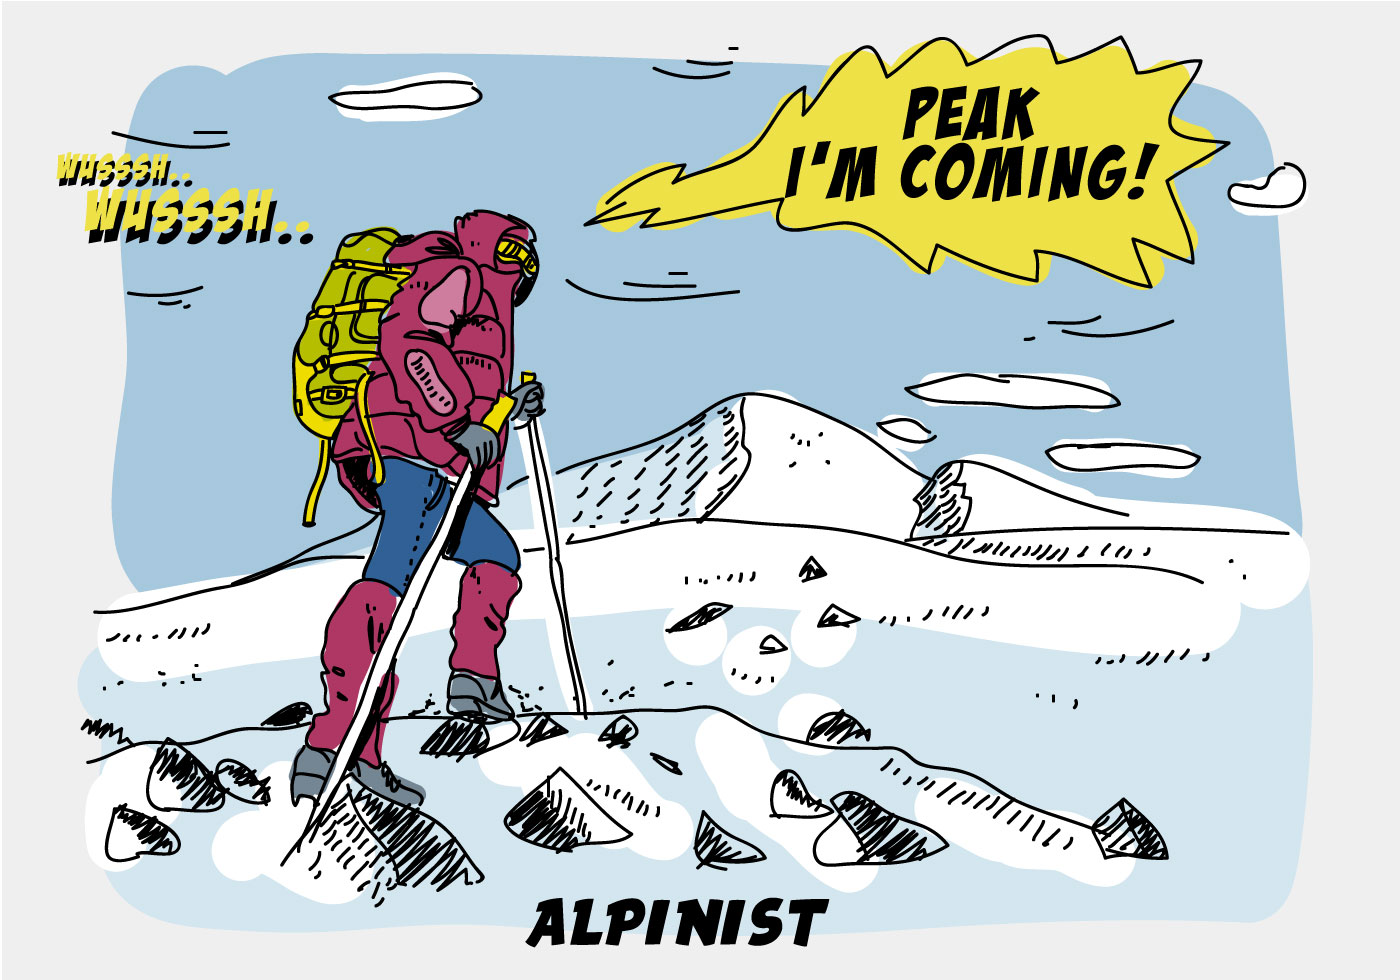
\includegraphics[scale=0.2]{files/alpinist-climbing-peak-mountain-comic-hand-drawn-vector-illustration.jpg}
\end{center}


Given the high number of quality applicants and a limited number of spots, in addition to having a good application profile, you want to show something that makes you \textbf{stand out}.  For example, even if you do not have research experience, you can talk about your personal projects, as long as they can help show you can do research. For example, if you have an open-source project that has lots of stars in Github, then you should mention it. If you often write technical, research-like blogs with many viewers, talk about them too.

There are other things you might not think are important but can make you stand out. For example, if you have a strong background in a non-CS field but can be integrated with CS, e.g., you have a degree or background in \emph{dance} or \emph{music} and want to integrate them with CS, do talk about it. Are you a female or a minority in CS (\autoref{sec:urm})? Do you participate in outreach activities that help increase diversity and inclusion in CS? Diversity is highly valued in CS programs in the US, and experiences in these areas can make you stand out and get noticed from reviewers.

\begin{commentbox}[Vu:]
In his \href{https://matt.might.net/articles/how-to-apply-and-get-in-to-graduate-school-in-science-mathematics-engineering-or-computer-science/}{post}, Matt Might was initially unsure about an application. However, upon learning that the applicant had led a 100km hike in the Himalayas, he decided to accept the applicant.  This is a good example of being \emph{stand out}, and I would also advocate for that student as this shows they have the persistence and determination required for research.
\end{commentbox}

% It is worth noting that in many cases,  an application could be rejected by most reviewers, however have a "champion", who doesn't even have to be in the Admission comittee, that strongly advocate for your profile.


\chapter{Funding}\label{sec:funding}
\chapterinfo{TAs, RAs, and fellowships are main funding sources for PhDs.  TAs are provided by the department to help with classes. RAs are given by profs. to help with their research.  Fellowships, provided by the university, department, or external sources such as government or industry, give move flexibility but can be very competitive.}

\epigraph{Bart, with \$10,000, we’d be millionaires! We could buy all kinds of useful things like…love!’}{\textsc{The Simpsons}}
If you're admitted to a \emph{good} CS PhD program, you should not have to worry about funding!
In the US, the common types of funding for PhDs are \emph{graduate teaching assistant} (GTA or TA), \emph{graduate research assistant} (GRA or RA), and \emph{Fellowship}.
RA is paid by a prof. for you to do their research. TA is paid by the dept. for you to help with teaching. Finally, fellowship is independent funding that can come from a school, a company, or an organization. \autoref{tab:funding} summarizes the differences.
Note that funding is typically more available for PhD students than
MS.

\begin{table}
  \centering
  \small
  \caption{Different types of PhD funding. All cover tuition, insurance, and stipend.}\label{tab:funding}
  \begin{tabular}{c|c|c|c}
    \toprule
    &\textbf{TA}&\textbf{RA}&\textbf{Fellowship}\\
    \midrule
    \textbf{From} & School & Profs. & School/External\\
    \textbf{For}                  & Teaching Assist.       & Research                        & Research                              \\
    \textbf{Cover All?} & Yes                      & Yes                             & Yes                                   \\
    \textbf{Summer?}              & No                       & Maybe                           & Likely                                   \\
    \midrule
    \textbf{Pros}                 & Research Freedom         & Get to do research              & Research Freedom                      \\
    \textbf{Cons}                 & Teaching Duties           & Research Restriction & Competitive, Limited             \\
    \bottomrule
  \end{tabular}
\end{table}

\section{Graduate Assistantship (TA/RA)}\label{sec:ta-ra}
The most common type of funding is \textbf{graduate assistantship}, which is either TA or RA. Both TA and RA come with tuition waiving (you don't have to pay tuition), health insurance (this takes care of your insurance, which is a must-have in the US), and most importantly, your stipend (i.e., your salary). Some universities also give significant discounts or pay insurance for spouses/children.

Several things about stipends.  First, the amount of stipend \emph{varies} and depends on factors such as location (e.g., a stipend in the DC area is likely higher than in Lincoln, Nebraska due to higher living costs). Second, an academic year (AY)  year is typically \emph{9-month} in the US, so the stipend is for 9 months. Third, you might get paid over the summer (\autoref{sec:summer-funding}) through funding from your professor or fellowship (typically no TA over the summer). Fourth, like most sources of income in the US, you will have to \emph{pay tax} on your stipend.  Finally, private universities might pay more for stipends, but they could have extra activity fees or some other hidden ones (e.g., you may need to pay some fees for each credit hour).

\paragraph{Low Stipend?} Students sometimes complain about their stipend being low. However, in most cases it is not bad, and you can live comfortably with it.  It might also be enough to support your spouse and kids (many CS PhD students have their families with them). So don't worry too much about the stipend.  If you're admitted to a good CS PhD program, you will be fine. A good school would know that it has to be competitive to attract students.  For example, at Mason, every year we try to improve the benefits, and especially stipend, for our graduate students.

For a full breakdown of how much a graduate student costs, see \autoref{sec:ra-cost}.


\begin{commentbox}[Vu:]
  TA and RA at Mason have similar benefits in tuition waiving and insurance.  The college and department will set the rate for a 9-month graduate assistant stipend.  TA, which is paid by the department, will likely be that amount but RA might be higher depending on the stage of the student (1st year vs ABD\footnote{All but dissertation: close to graduate.}) and the prof.
  \tcblower
  Having health insurance is required at many US universities.  Do not assume that you're young and healthy and ignore insurance (\autoref{sec:cultural-misc}).  At Mason, and most CS PhD programs, your GTA or GRA comes with full insurance. In fact, at Mason your spouse/children will get a significant discount rate for health insurance.  So you will never have to worry much about health issues for you or your family here.
\end{commentbox}


\subsection{Teaching Assistant (TA)}\label{sec:ta}

TA is common in the beginning when you haven't found an adviser who would pay you RA. It is also common to sandwich between TA and RA (e.g., when your prof. does not have sufficient funding or you want to try the TA experience).

Your TA is paid through the school or department, i.e., they hire you to help teach.
As a TA, you spend up to 20 hrs/week and help with classes (e.g., grading or teaching labs/recitation).
During a semester, a TA might work with several courses and professors (not necessarily their adviser).  TA funding is \emph{not} typically available during the summer (\autoref{sec:summer-funding}), which has few courses.

\paragraph{How to get TA?}  Unless you have other funding such as RA or fellowships, TA is typically the default for CS PhD programs. In your application, just simply indicate that you need financial assistance. Typically, adcom will either admit you and give you TA, or reject you. We do not admit a student without supporting them (\autoref{sec:ievaluate}).

\begin{commentbox}[Vu:]
  At Mason CS, admitted PhD students have 4 years of GTA guaranteed, and also receive a stipend for the first summer (\autoref{sec:summer-funding}).
\end{commentbox}

Even if you have other funding and do not need a TA, you still should do TA at least once.  This allows you to see what teaching is like, which is especially helpful for a research career where you often give talks and tell people about your work. Mason sometimes has classes that a more senior student can teach.  In that case, you will be paid as GTA or even sometimes as a lecturer.  This is a good opportunity for students to get teaching experience and you might even get paid a bit more.

\subsection{Research Assistant (RA)}\label{sec:ra}
RA is provided through a professor through their funding so you can work on their project.
You do not need to teach as an RA, so you can focus on your research. Depending on the professor, RA may be available during the summer. \autoref{sec:ra-cost} gives more details on RA budget.

\textbf{How to get RA?} When a professor recruits you, they might offer you an RA right away (so you start with an RA).  However, a more common scenario is that you first get admitted with TA, and then after a year or two find an adviser to support you with RA.

It is important to note that RA is \emph{never guaranteed} as it depends on the funding situation of the prof. So you should also pay attention to TA, which is a good backup plan (remember, typically TA and RA have quite similar benefits). This means you should also check if TA is readily available for PhD students in the program.


\begin{commentbox}[Vu:]
  If you got recruited and offered an RA by a prof., you will likely get admitted.  For example, if a prof., even if not in PhD adcom, wants to fund you, adcom will likely respect that decision and admit you.
\end{commentbox}

\section{Fellowships/Scholarships}\label{sec:fellowships}

Fellowship is another type of funding that students can get from the university, industries, or government.
Fellowships are typically competitive and generous, giving pretty much all benefits tuition/insurance that a TA/RA has.  They might even give higher stipends (including summer) and open doors for job opportunities such as internships.

\textbf{How to get Fellowship?}   Many schools provide fellowships to attract students. You likely will not need to do anything and adcom will recommend such fellowships to strong students. Some schools automatically offer a fellowship to all accepted students, while others only award it to a limited number of admitted students, such as the top percentile.

For external fellowships including those from the US government (e.g., NSF, DOD) and tech companies (e.g., Google, Microsoft, Facebook), you will need to apply.  % However, tech companies including Google, Microsoft, Facebook have fellowships that international students can apply for.
Prestigious external fellowships typically require a clear and good research plan (the GRFP also requires outreach activities and plans). So it might be a good idea to wait until your second year to have research experience and even publication before applying. Remember, you're competing with the top PhD students at top universities worldwide.

\begin{commentbox}[Vu:]
  PhD applicants at Mason are automatically eligible for a \emph{Presidential Fellowship}.  It is at least as good as GTA but the most important thing is that as a fellowship it is truly free money (i.e., you do not depend on any prof. or TA).  Adcom members nominate applicants for this fellowship and the whole committee will decide.
\end{commentbox}

In addition to general fellowships that are available to all students, there are also specific fellowships, e.g., for US citizens and permanent residents (\autoref{sec:domestic-students}), for underrepresented minority (URM) students (\autoref{sec:urm}), and students from specific countries. There are many fellowships available, so you should look for them and apply.

In general, fellowships, especially those that are open to everyone, are highly competitive and prestigious, and you will stand out if you get one.  Every PhD student has pubs, but only a few would have NSF Graduate (GRFP\footnote{\url{https://www.alexhunterlang.com/nsf-fellowship} is a good starting place for the GRFP with lots of proposal examples.}) or Microsoft fellowships. In fact, these are so prestigious that even if you didn't get it but make it to the final round or even \emph{``honorable mentioning''}, your school will still mention you on their website, and you should put it on your CV.

\section{Miscs}

\subsection{Funding In the Summer}\label{sec:summer-funding}

One confusion students often have is whether they will get paid over the summer.  This depends on the funding source.
First, recall that an academic year (AY), which consists of Fall and Spring semesters, is typically 9 months, so your stipend is for 9 months (and many places allow you to spread it over 12 months).

If your funding source is TA (\autoref{sec:ta}), you typically do not get paid over the summer, which has few courses.
Some CS departments offer summer funding, but it is not guaranteed and might not be a lot. For example, at Mason, we offer summer funding for 1st-year PhD TA students. The amount over the 3-month summer is similar to their monthly stipend (i.e., their 9-month stipend divided by 3 for the 3 summer months).

For RA (\autoref{sec:ta}), it depends on your prof. and their funding. When writing grant proposals, profs. typically include summer funding for their students (\autoref{sec:ra-cost}). However, funding is never guaranteed, e.g., the prof might not get the grant.

\begin{commentbox}[Vu:]
For my students, I have been fortunate to have funding to support them over the summer. Over the 3-summer months, I typically pay them 1/3 of their 9-month stipend. I prioritize summer funding for my students because Mason has very good TA resources so they never have to worry about funding during the AY.
\end{commentbox}

Finally, for fellowships (\autoref{sec:fellowships}) you might get paid over the summer depending on your fellowship (\autoref{sec:fellowships}). Good ones, e.g., from NSF, Google, and Microsoft, will pay you the whole year.

\subsection{How much do you cost?}\label{sec:ra-cost}
\sectioninfo{Your entire PhD program costs about \$400K in total, but you \emph{do not} pay for it.}

PhD students often ask why their salary is low compared to the large grants their advisers get. They also wonder why their offer letters sometimes show that their benefits are higher than what they receive (i.e., stipend).

\begin{center}
  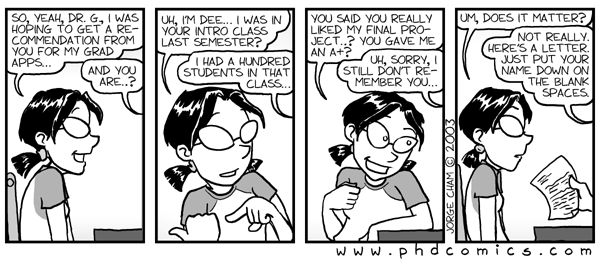
\includegraphics[scale=0.5]{files/c6.png}
\end{center}

\begin{table}
  \centering
  \small
  \caption{GRA cost breakdown. F \& A is Facilities \& Administrative Cost Base and
    MTDC is Modified Total Direct Cost. These are things that the university can charge overhead to.}\label{tab:cost}
  \begin{tabular}{rcl}
    \textbf{Budget} & \textbf{Cost \$} & \textbf{Notes} \\
    \midrule
    GRA (9-month) & 30K & \\
    GRA (summer)  &10	& 3-month, 20hrs/week\\
    \textbf{Total Salary} &\red{40K}	&\\
    \midrule
    Health Insurance	&3K	& full year\\
    Tuition (In-State) &	15K	& (\$680/ Credit + \$150/Student Fee/ Credit)* 9 credits = \\
                    &&\$7470 (\$6120 + \$1350) per semester\\
    \textbf{Total Tuition \& Insurance}	&\red{18K}	&Full year tuition + insurance\\
    \midrule
    Conference Registration	& 500 & \\
    International Travel &	1800& \\
    Domestic Travel	& 700	& \\
    \textbf{Total Travel}&	\red{3K}	\\
    \midrule
    Total Direct Cost	& \red{61K}	&Salary + Travel + Health + Tuition \\
    F \& A (MTDC)	& 21K	& Direct Cost - GRA Salary\\
    Total Indirect Cost	& \red{12K}	&58.9\% of MTDC\\
    \textbf{Total (Direct + Indirect)} &	\red{73K}	& Budget for a GRA\\
    \bottomrule
  \end{tabular}
\end{table}

\autoref{tab:cost} shows the budget breakdown for a GRA per year.
These numbers are based on my experience at public universities in the US. Private universities may have different numbers.  For simplicity, I will assume the department has a 9-month stipend of \$30K and a 3-month summer of \$10K (a third of the 9-month stipend). I will also use Mason tuition rate of about \$15K/year for full-time study (which is quite cheap compared to private universities, e.g., Univ. of Chicago is a whooping \$70K) and a 58.9\% rate on \emph{indirect cost}, which is a typical rate charged for overhead or administrative costs (yes, after all, universities are businesses!).  Finally, I assume the students take two conference trips per year, one domestic and one international (conf. registration, airline tickets, taxi, meals, etc are all included).

In the end, the total budget comes out to be \$73K/year to support a PhD student. \emph{The summary is that over your 5--6 years of your PhD, you cost about \$400K, and while your stipend is X, your adviser probably pays 2X for you}. But of course, the nicest thing is that you do not have to pay for any of this! You get to gain the knowledge, do research, travel, (and don't even have to buy any research or computer equipment as mentioned in \autoref{sec:buying-equipment}) and also get paid!



\chapter{Choosing Schools and Professors}\label{sec:schoolsandprofs}

\chapterinfo{Not every university has PhD progarms in CS. Not every professor, even those in CS, can advise or graduate CS PhD students.}

\epigraph{\vspace{-0.2in} The answer to life's problems aren't at the bottom of a bottle. Heh heh! They're on TV!}{\textsc{The Simpsons}}


Choosing a school and an adviser is clearly among the most important things in your mind when you apply and especially when you get admitted.  This is further complicated due to cultural differences and the unfamiliarity of international students with the US higher education system.  This section aims to mitigate some confusion and help you make informed decisions.

\section{Choosing a University}\label{sec:choosing-university}
\sectioninfo{Select schools based on their CS program and faculty research interests.}

We will first discuss universities in the US that offer PhD in CS. Then we will talk about how to select them.

\subsection{Schools that offer PhD in CS}

Most US universities have CS studies, but many of them do not have a PhD program in CS. These universities might offer just Bachelor's degrees (e.g., BS) and no graduate studies (i.e., no MS or PhD degrees), or they just offer MS programs (but no PhD). For example, Penn State in University Park has PhD in CS,  but Penn State in Harrisburg only has BS and MS in CS, and Penn State in York only has BS in CS.  On the other hand, multiple locations of the University of Texas, e.g., Austin, Dallas, and Arlington, have PhDs in CS.

Thus, if your goal is PhD in CS, you have to aim only for schools offering such a degree.  %This might sound obvious but many students (even those in the US) get confused due to the large number of universities.
While this can be confusing due to the large number of universities in the US, a little research, e.g., searching for PhD in CS from the school website, will help you find out. Schools listed in \autoref{sec:ranking} have PhD programs in CS, so you can start there.

% \subsection{R1, R2, ...}

\subsection{Selecting and Ranking Schools}\label{sec:selecting-ranking-schools}
\begin{center}
  
\includegraphics[scale=0.5]{files/c1.png}
\end{center}

Many students just put schools into two bins: (i) top schools that they dream about, and (ii) everything else.  They commonly use rankings from US News, which is not transparent and questionable\footnote{\url{https://cra.org/cra-statement-us-news-world-report-rankings-computer-science-universities/}}.  Sometimes they evaluate based on the reputation of the school's undergrad program or the reputation of the school's non-CS programs such as medical, math, or physics.
Many international students rank universities based on popular places they know in the US, e.g., California, Texas, and New York.

Instead of these superficial criteria, you should specifically consider the CS program and the research interests of faculty members.
You can learn about these using resources such as \href{https://csrankings.org}{CSRankings.org}. You will be very surprised to learn that a school that you didn't know much about can have very strong research in your topic (and vice versa, a school you thought highly about might have no faculty working in the research field you're interested in). This is also a good way to learn about individual faculty, e.g., who works on what, and well-known CS conferences\footnote{In CS (and probably only in CS), conferences, not journals, are often the main venue to publish research findings (see \href{https://homes.cs.washington.edu/~mernst/advice/conferences-vs-journals.html}{why here}).}. %\autoref{sec:ranking} gives the top 50 CS programs in the US according to CSRankings.

\begin{commentbox}[Dat:] Most Vietnamese students, including those from top schools, \textbf{do not know} about CSRankings.  Maybe applicants who worked at top research places such as VinAI would know about it.
\end{commentbox}

\paragraph{What matters to you?} While many find CSRankings useful, it is still superficial as every other ranking.  You should consider other factors that matter to you.  For example, you might prefer places with a large community from your country (e.g., Northern VA has a large population of Vietnamese). You might prefer places with high-tech companies (Seattle or Silicon Valley), with many outdoor activities (e.g., hiking, skiing), or with better weather (\emph{``PhD can be depressing, so would you rather be depressed in California or New York?''}).  You might need to think about the cost of living, e.g., living in California is more expensive than in Virginia, or places with high crime rates (note that while some universities might be in a high-crime city but the campus itself is safe).

If you get admission to several places, you should consider attending Open Houses (\autoref{sec:accepted}) and contact profs. that you're interested in at those places and talk to them.  They would be more willing to chat with you now that you have been admitted.  Ask questions about \href{https://github.com/dynaroars/dynaroars.github.io/wiki/Answers-to-Ph.D-Advisor-Guide}{their work}, how they manage students, and their expectations. You can even ask to contact their students.

\begin{commentbox}[Hung:]
  I always encourage the students I admitted to talk with my students and the students of other faculty in other schools who admitted them. You will unlikely hear straight-out complaints from current students in a prof’s group. But sometimes what is important are things that they (current students) don’t tell you. Pay attention to their ``level of excitement'' being in the group.
\end{commentbox}

\begin{commentbox}[Xiaokuan:]
  Chinese students often only look at US News rankings when selecting their PhD universities (I did that, too, when I was applying for PhD positions).
  Now that I am a professor, I find it to be the least promising way.
  %
  The reason is that US News does not provide a good metric for evaluating the quality of the PhD program.
  %
  If you want to do great research, CSRankings is the best way to find good and active professors (which did not exist when I was applying),
  since it solely focuses on publications at top-tier CS conferences.
  %
  Also,
  I think PhD is not only about research;
  you need to also consider your daily life there since you will (probably) stay for at least five years.
  %
  You might regret it if you did not consider this seriously before applying.
  %
\end{commentbox}


\subsection{PhD in other related fields: CE, IST, Cybersecurity}\label{sec:related-fields}

You \emph{do not} need to do a PhD in CS to work in CS areas. For example, in addition to a traditional CS department, Mason has IST and Cybersecurity departments, both of which have faculty with PhD in CS and work on CS topics (e.g., AI, Security, Robotics).  So you still can do CS research and publish in CS-focused venues even if you're not in a traditional CS program.  It is common to see faculty with PhD in CS in a non-CS department as well as faculty with non-CS PhD in a CS department.

However, if your goal is a PhD in CS, then you need to be in the CS dept \emph{and} advised by a CS faculty. A non-CS faculty can serve in the PhD dissertation committee (common) or \emph{co-advise} (somewhat rare), but your main PhD adviser will likely be a tenure-line faculty in CS (\autoref{sec:faculty-types}).
For example, a prof. in Stats or Math might be able to serve as a co-adviser, but not as a sole adviser of a student in a CS PhD program. 
If in doubt, check with the CS department for their requirements.

For this specific reason,  CSRankings includes only faculty who can advise CS PhD students. I also have compiled a \href{https://github.com/dynaroars/dynaroars.github.io/wiki/Viet-CS-Profs-US}{list} of Vietnamese faculty who can advise PhD students. \autoref{sec:faculty-types} talks more about who can serve as your PhD adviser.


\section{Choosing an Adviser}
\sectioninfo{The best adviser is the one that you can work well with. But you do not know that until you start working with them.}


There is no one-size-fits-all answer to this question. The best adviser is the one that you can work well with.  But how do you find such a person?

Fortunately, while some non-US programs require finding an adviser and research topic before starting the PhD (\autoref{sec:non-us-differences}), CS PhD programs in the US will typically give you a couple of years to ``shop'' for advisers and research topics.  This is especially true if you're admitted with TA (\autoref{sec:ta}), which gives you time to explore and find an adviser.

\subsection{Finding an Adviser}

Assuming you're not familiar with any particular one, then first search for profs. that share similar research interests.  For example, in CSRankings, if you want to work with PL, you can search for those published in PL conferences.  If you want to work with SE \emph{and} AI, you can search for faculty who work in both SE and AI.  Then you research about that prof. (e.g., go to their website) and contact them (\autoref{sec:contact}).

\begin{commentbox}[Xiaokuan:]
  Whether the student's research interest matches that of the adviser is very important;
  if there is a mismatch,
  either the student or the adviser has to make compromises,
  which often leads to disagreements or conflicts.
  IMO, the adviser should be the one who \emph{guides}  students to do research while allowing students to pursue their own interests,
  instead of \emph{dictating} their research.
\end{commentbox}


Another way is taking graduate-level courses in the topics you are interested in.  Many profs teach \emph{special topics courses} and \emph{research seminars}, and they might be recruiting students. Do well in the class, answer questions, talk to the prof. after classes, etc---being stand out.  Many profs, including myself, prefer taking in new students this way.  It gives both the prof and student more time, e.g., a whole semester, to work and evaluate the relationship before making any commitment (sounds like a marriage!).

You can also ask to do an independent study or research with a prof. This can be informal (no credits) and takes place during the summer or winter break.  For example, I do this with several students, some of whom are undergrads. Many will drop out because they find they don't like my research, but some find that they like the work.

Ultimately, choose a prof. that fits you by communicating with them, taking their courses, meeting and asking them questions, and talking to their current students. It will take time and effort, but since you will be working with this person for 5+ years, it is important to try to find the right one.

\begin{commentbox}[Thanh:]
  In my opinion, having a well-suited adviser is crucial for a successful PhD and research career. One effective approach to finding a suitable professor is by working with a professor during your undergraduate studies. An exemplary instance is VinAI's residency program, where residents collaborate with professors from the US for two years before applying to PhD programs. Many VinAI residents have achieved remarkable results and gained admission to prestigious US universities. Unfortunately, VinAI's resident program is limited to AI research.

  In other fields, e.g. Software Engineering, Vietnamese students face challenges in reaching US professors. Do you have any tips for Vietnamese students who want to connect with US professors and work as research assistants?
  \tcblower
  \textbf{Vu}: \autoref{sec:contact} shows how to contact a professor for research opportunities. Many will say no (or do not reply) as they do not have the bandwidth to take on random students, but some may say yes if they see a potential fit.
\end{commentbox}

\subsubsection*{Additional Resources}
\begin{itemize}
  \item \href{https://www.cs.columbia.edu/wp-content/uploads/2019/03/Get-Advisor.pdf}{The Definitive ``what do I ask/look for'' in a PhD Adviser Guide}
\end{itemize}
\subsection{Who can serve as a PhD adviser?}\label{sec:faculty-types}

\emph{Not} every faculty can serve as your official PhD adviser. Let's try to understand the different types of faculty and their roles. For example, you might hear about tenured,  tenure track, and teaching faculty.  You might also hear about assistant, associate, full, adjunct, emeritus, teaching, and research professors. Here is a primer on these terminologies.

\subsubsection{Types of Faculty} There are typically two types of faculty at an R1 research university: tenure-line and teaching.  The main difference is their focus: research, teaching, or both. Tenure-line faculty are typically more research-focused and can mentor PhD students, while teaching faculty are more teaching-focused and typically do not advise PhD students. Thus when contacting a prof. for research opportunities (\autoref{sec:contact}), you should focus on tenure-line faculty (and not adjunct or emeritus :p).

\textbf{Tenure-line faculty}, consisting of tenured and tenure-track profs., focuses on research, which includes publishing papers, obtaining grants, and mentoring PhD students.  They often have a low teaching load, e.g., 1 course per semester. \emph{Tenured} faculty are professors who have been promoted to permanent positions (informally, very hard to fire them).  \emph{Tenure-track} faculty are professors who are on the track to get tenure.  For most schools, tenure-line is the main type of faculty that can serve as a formal adviser of PhD students. \autoref{sec:tenure-vs-tenure-track} talks more about choosing between tenure and tenured-track professor as your adviser.

\textbf{Teaching faculty}, sometimes called instructional faculty or professor of practice, mainly focuses on teaching. They typically teach 3--4 classes per semester (which is quite a lot) and \emph{do not} have research responsibilities, e.g., they do not have to worry much about publishing papers or obtaining grants. As such they typically do not have funding (e.g., RA~\autoref{sec:funding}) to support PhD students.
Depending on the university, they might be able to \emph{co-advise} and mentor PhD students with a tenure-line faculty, but they typically do not formally advise and graduate PhD students.

Note that at many universities do not allow \emph{non-CS profs}, even tenure-line ones, to solely advise and graduate PhD students in CS (see \autoref{sec:related-fields}). 

Some universities have \textbf{research faculty} or research scientists, who are typically non-tenure line faculty and focus on research (e.g., publishing papers and getting grants). 
They can recruit students and provide RA funding for them. 
They can also teach classes but typically have a lower teaching load.
For some universities, they \emph{can} solely advise and graduate PhD students, but for others, they cannot. 

\textbf{Adjunct faculty} is not full-time, e.g., they might be working in industry and teach a class or two for fun. \textbf{Emeritus faculty} means they are retired from the university, e.g., they could move to the industry, but still have some affiliation with the university.   Due to their roles, these profs. typically do not advise PhD students.


\subsubsection{Ranks} Faculty have ranks such as assistant, associate, and full, regardless if they are tenure-line or teaching.  Assistant means new faculty, associate means they have been promoted (or was hired after being in the industry for a while), and full means they are senior. 

Typically, a tenure-track faculty starts with being an assistant professor and then gets tenure and promoted to associate (around 6 years). Note that getting tenure is a huge deal, and it might change the way they work with students, e.g., they might be more relaxed and less stressed (\autoref{sec:tenure-vs-tenure-track}).

After that they go up for full prof. (time varies, some become full within 3--4 years, some 10+ years, some remain associate). A non-tenure track faculty, e.g., teaching or research faculty, also starts with Assistant, then is promoted to Associated, and finally Full.




\subsection{Tenured or tenure-track faculty?}\label{sec:tenure-vs-tenure-track}

\begin{center}
  
\includegraphics[scale=0.4]{files/c8.png}
\end{center}

Now that you know a bit about tenured and tenure-track faculty (\autoref{sec:faculty-types}).  Which one should you choose as your adviser? 
Either can be a good adviser, but they have different strengths and weaknesses.


Tenure-track faculty, e.g., assistant professors, are likely young and active in research (they have to, to get tenure). Thus, they will devote more time to work with you and push you to do research and publish. However, you might not be too independent when you graduate because they have been too hands-on with you.  Also, they may not have as much experience in managing students and may not have as much funding (yet).

Tenured faculty, e.g., associate and full profs., are likely older, more well-known, and have more experience in managing students.  However, they might not push you as hard and expect you to figure things out yourself, i.e., you need to be independent.  Some tenured faculty are also no longer active in research and are more involved with administrative responsibilities or with their startup companies (this means they will likely not take new students). \autoref{sec:faculty-types} gives more details on faculty types.

% \subsection{Strong Faculty vs High-ranked School}
% \begin{commentbox}[Thanh:]
%   When considering PhD programs, we often wonder if we should prioritize a high-ranking university or a professor with a strong reputation? Of course, both are great, but it is hard to achieve both.  I believe receiving some guidance from you  would be incredibly valuable.
% \end{commentbox}

% This is a good question and there doesn't seem to be any best answer or specific algorithm that you can use.  But I'll throw out something for you to think about. To me, there are many good schools in the US and so you have some leeway in choosing.  For example, I don't believe there's much difference among schools in top 5 (e.g., CMU, UIUC, UCSD, MIT, GTech are in the same equivalent class), top 10 (e.g., Michigan,  Stanford, UWash, UC-Berkeley, Cornell is another equivalent class), top 20, top 30, top 40, and so on (though I would say schools above 100 are pretty much in the same equivalent class).  It's hard to say a top X is much much better than a top X+20 (e.g.,  Purdue at 15 is stronger than Yale at 35, but not \emph{that much} stronger as you would think).  So keep that in mind, while ranking does matter (e.g., more active faculty, stronger students), the lower ranked universities are still pretty good, might have sub fields that are extremely strong (NCState is 40th, but in Software Engineering it is easily top 5), and many unique things.  This is in contrast with universities in Vietnam where there are large gaps among the top 5, 10, and so on.


\section{Contacting a prof. How to get a desired reply?}\label{sec:contact}

\sectioninfo{Individually faculty member \emph{cannot directly admit} a student---so do not email and ask if you have a chance. However, faculty can \emph{advocate} for a student and therefore increase their admission chance---so do contact and introduce yourself.}


\begin{center}
  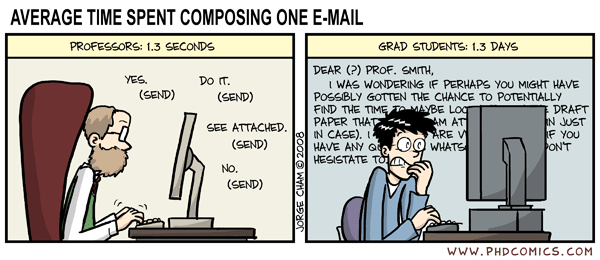
\includegraphics[scale=0.6]{files/emails.png}
\end{center}


Faculty often receive ``cold'' e-mails from prospective students. Most of the time, we ignore these emails, but on some rare occasions, we do answer them. So how to write an email that gets our attention?

First, if you want to contact a prof. to \emph{ask about your admission chance}, please \textbf{don't}. We don't know and can't answer because as explained in \autoref{sec:evalapps}, we don't make individual decisions and might not even be assigned to evaluate your application.  It is the same as sending a paper draft to a journal editor and asking them if your paper has a chance.

So how to get someone to look at your profile and give input? You could ask your professors, LoR writers, collaborators, or those who have previously applied. For this kind of feedback, ask someone you have a personal connection with.

On the other hand, if you want to contact a prof. to ask about \emph{research opportunities}, or \emph{GTA/GRA} support, then \emph{yes}, I believe you should---it is \emph{worth it}. However, you really need to put effort into it and do it the \emph{right way}.

First, read the prof's website, and see if they say something about contacting them. Many profs. explicitly state how prospective students should (or should not) contact them, e.g., using specific email subjects.
In general, the best way to catch the prof.'s attention is to \emph{customize your email} for them.  For example, read their papers, know what they work on, and see if you are interested in their research. Then email them and talk about how/why their work would match yours.
In contrast, if you write a generic email that can be sent to multiple professors (e.g., if you just change some names and keywords in the email or copy and paste paper titles), you will not get a response.

Below is a good example that I would likely reply.

\begin{commentbox}[Dear Prof. Nguyen,]\\

  I am writing to inquire about potential research opportunities as a GRA in your group at Mason. Currently I am an undergraduate student in Computer Science at UNIV and plan to graduate in May 2023.
    \\

  I have read your TSE'21 paper on numerical invariant generation, and I am interested in this line of dynamic invariant research. I have worked (optional: with prof. Y at Z) on static program analysis and I think it could be used to tackle the spurious issues mentioned in your paper. I have a short paper at conference/workshop C and a project on symbolic execution (Github repo G).

  ...

 \tcblower
  This is a good example because it is written just for me.  It shows that the student knows about my work on invariant generation and has a related background (paper C and project G).
\end{commentbox}

Finally, profs. are very busy so don't take it personally if you don't get anything from them (though I would be very surprised if such thoughtful emails get no replies!).
See~\autoref{sec:kiss-of-death-emails} for common mistakes in emails and~\autoref{sec:interpreting-response} for interpreting replies.

\begin{commentbox}[Xiaokuan]
  Applying for PhD and contacting a potential PhD adviser is a classic \textbf{`why me, why you'} problem,
  similar to looking for a job in a company.
  On a high level,
  you need to show that you have done your \emph{homework}
  regarding the professor and the university,
  and clearly explain:
  1) why do you think you are a good fit in professor A's group?
  2) why do you want to be advised by professor A, not B?
  3) why do you want to apply for university X, not Y?
  If you don't want to spend time doing your homework,
  the chance of getting a reply is close to zero.
\end{commentbox}


\begin{commentbox}
  [Deepak:]
  In my view, cold emails are not welcome by most faculty members and should be avoided. However, if one is already admitted to a program in some department, by all means, email the faculty you may be interested in working with, but do mention right at the beginning that you are already admitted to the program as well as several other universities. State specific areas (preferably specific topics-ML, robotics instead of AI).
\end{commentbox}



\subsection*{Additional Resources}
\begin{itemize}
  \item \href{https://yonatanbisk.com/emailing_professors.html}{A Note about Emailing Professors} by Yonatan Bisk
  \item \autoref{sec:accept-postpone-decline} How to accept/postpone/decline PhD offers (and do it gracefully)
\end{itemize}


\subsection{Kiss of Death in Emails}\label{sec:kiss-of-death-emails}

\begin{itemize}
    \item \textbf{Send emails to the wrong prof.}. Most students often do not pay attention or know about this, but a very common reason why you don't get a reply is that you send email to profs. who do not / cannot advise CS PhD students (e.g., adjunct, emeritus, teaching, non-CS, etc.). See \autoref{sec:faculty-types} for details. While these profs. might be able to co-advise, they typically do not have the bandwidth, funding, and the desire to mentor students for research (they are already overloaded with teaching and other service duties). So do some homework before sending emails, e.g., most CS profs. who are active in research will have a website with their work (publications) and students; some also have lab website dedicated to their group. Most teaching and adjunct profs. do not have such a research page.
        
    \item \textbf{Generic}. You should already know this! A copy and paste kind of email or those that can be sent to multiple ppl with very little modifications show the lack of interest and will be treated as spam. Most likely we will not reply to these emails. 

    \item \textbf{Self-focus}. Focusing too much about you and your achievements but not why you are interested in the prof.'s work (\autoref{sec:contact}). Mention why you're interested in their work and how your background can contribute. 

    \item \textbf{Too long}. Keep it to about 3--4 short paragraphs. Less is more and too long emails are often not read and discarded. Don't attach course transcript or test scores in the first email. If they are  interested they will ask for them.  Attaching CV is OK. Sample papers and links to your Arxiv papers or GitHub projects are also OK if they are relevant.
    
    \item \textbf{Flowery greetings and language}. Don't use ``Dear esteemed professor'', don't ``hey there''.  Do not call the prof. by their first name in the first email (some don't care but you don't want to take the risk -- you don't know them that well yet).  Do not use Mr., Mrs., etc. To be safe, use Prof. Lastname or Dr. Lastname (\autoref{sec:address}).
    
    \item \textbf{Ignoring the Prof's guideline} and asking questions that are already answered on their website.  Many profs. put very specific information on how to contact them on their website (e.g., email subject, what to include).  Following this helps you stand out and increase your chance of getting a reply.
    
    \item \textbf{Fancy format}.  Do not use colors, fancy fonts or formats. While not really a kiss of death, it is very annoying, especially for ppl in CS (and probably many other fields) who often prefer plain messages.
    
    \item \textbf{Mass emails}. I've seen it many times when a student mass emails all profs in a department (e.g., through CC or even BCC---we know because faculty talk to each other).  This will result in no reply or a very harsh one on how unprofessional you are.
    
    \item \textbf{Don't CALL}. Not related to email but sometimes students get desperate and call the prof.  This is a big no-no, especially for CS ppl who often prefer email over phone calls. Seriously though, don't call any prof. unless they ask you to. 
\end{itemize}




\subsection{Interpreting Response}\label{sec:interpreting-response}
Even if you avoid the kiss of death emails (\autoref{sec:kiss-of-death-emails}), you might still not get a reply.  This is very common and you should not take it personally.  There are many reasons why you might not get a reply, e.g., the prof. is not interested, they are too busy (\autoref{sec:busy}), they are not taking students, they are on vacation, etc.  Here are some common responses and what they mean:

Some generic responses are:
\begin{itemize}
\item \textbf{No reply}. This is by far the most common response (see why in \autoref{sec:busy}).  It means they are not interested.
You might try again in a few weeks or months, but don't expect a reply. And after a couple of tries, you should move on.  It simply means they are not interested.
\item \textbf{Not taking students but encourage you to apply}. Polite way of saying not interested and referring you to the admission process. Note that this does not in any way mean that they think you have a good chance of getting admitted.

\item \textbf{Not taken student this year (but encourage you to apply next year)}. Polite but generic response.  And like the previous one, encouragement to apply does not mean they think you have a good chance of getting admitted.

\item \textbf{Come talk to me after you're admitted}. Generic. Refer you to the admission process. But if you get admitted then you can reply to them and say you're admitted and would like to talk.

\item \textbf{Cannot admit you directly. Need to go through admission process}. Generic. They are not interested and refer you to the admission process.

\item \textbf{I am not taking students but I co-advise/can serve on your committee} While this might sound good, it's generic because it says once you're admitted and have an adviser, then contact me again. 

\item \textbf{I am not taking student but Prof. X might be}. Not common as most profs. will not refer you to their colleagues. However, this is better than the previous responses. While they cannot take you, they think you are a good fit for X. So follow up with a thank you and say you'll contact X.  And then contact X and say that Y referred you to them.
\end{itemize}

In short, all of these replies mean the prof. is not interested.  The best positive response is that they want more information from you, e.g., your CV, transcript, paper, or a chat (like an interview). 




\section{Are profs. so busy that they completely ignore emails?} \label{sec:busy}

Profs. are busy. We have many deadlines, meetings, and emails, many of which are from prospective students looking for research opportunities. we also have a life outside of work, e.g., family, hobbies, etc. 

However, this is not why we ``ghost'' you and provide no response.  It is because we want to avoid misunderstandings.  A response (\autoref{sec:interpreting-response}), no matter how clear we think it is, might be misinterpreted by the student.  For example, if we say we are not taking students but still (strongly) encourage to apply, then the student might take it as a positive sign of admission. Or if we say we are not interested, the student might take it as a personal rejection and not apply at all.  So it is not because we are too busy to reply, but because we do not want misunderstandings and have to deal with them later. 




\begin{commentbox}{Vu: }
    I skim through \emph{every email} sent by students for admission and research opportunities (many of which are from undergrads and highschool students). So that means I do read your email, and it doesn't go to my spam/trash folder. 
    However, I only reply to those that I think are a good fit and ask them to chat with me.
    \end{commentbox}
    

\chapter{Miscs and FAQs}\label{sec:faqs}

\epigraph{``I want to share something with you – the three little sentences that will get you through life; number 1: Cover for me, number 2: Oh, good idea, Boss, and number 3: It was like that when I got here.''}{\textsc{The Simpsons}}

%\section{"Chance me" questions}\label{sec:chance-me}

%Reddit and other grad admission forums are full of ``Chance me'' and ``roast my profile'' questions. These are questions where students post their profiles and ask others to evaluate their chances of getting admitted to their choice of schools.  

%These questions are not useful and should be avoided. First, no one knows! Even adcom members can't tell if you would get admitted to their programs or not. As mentioned throughout this guide, the admission process is complex and involves many factors that are not part of your profile, e.g., whether the faculty have funding or are interested in your background. Second, answers to this questions are often not helpful to you.  Faculty and people knowledgeable about the process will not answer these questions, and those who do are often not knowledgeable and might give you false hope or despair. OK, someone say your GRE is low (which does not even matter for most schools (\autoref{sec:standard-tests}) , are you going to retake it?  Or someone says your GPA is low, are you going to apply to a different school?  No, you should apply to the schools you want to go to and see what happens.  If you don't get in, then you can ask for feedback and improve your profile for the next round.






\section{How long does it take to evaluate an application?}\label{sec:ievaluate}
\sectioninfo{It takes me about 10--15 minutes to review an application.}

On average, I spend about 10--15 minutes reviewing each application (less for clear rejections and more for potential acceptances). While this seems short, it is not that difficult to tell if an application is good or bad.  In fact, this
is twice what other faculty spend on average, e.g., Philip Guo spent \href{https://pg.ucsd.edu/PhD-application-tips.htm}{3--5 minutes} per application.

For each application, our system compiles a single PDF file, which consists of a summary (degrees, GPAs, etc), transcripts, test scores, LoRs, a CV, SOP, and writing samples. I usually read in this order. I start with the \emph{summary}, checking for low GPAs or test scores below the university minimum (\autoref{sec:standard-tests}). I then skim the \emph{transcripts} for low grades in relevant courses, noting issues like ``many low grades in main courses or unknown international school with good GPA''.  These are not as important as LORs or SOP but I read them first because the review system has questions about them (e.g., ``is GPA good? is IELTS sufficient?'')

I read carefully \emph{strong LoRs} and skim weaker ones, noting either strong letters from well-known professors/researchers or generic content. I skim over \emph{CV} and look for publications, research experiences, and notable achievements. I take notes of things like ``published papers in top venues'' or ``gold medal in an international competition''.

I skim weak \emph{SOPs} but read strong ones thoroughly. I note whether the SOP is exciting, research-oriented, standing out, e.g., applicant is minority (\autoref{sec:urm}), and tailored to our program (e.g., if they are familiar with the work of some faculty or have talked to them). These notes are entered into the evaluation system.

Finally, I enter my decision, which is usually either a rejection or an offer of admission with full funding (e.g., from TA). I also recommend very strong candidates for the University Presidential fellowship. Note that while the system has other decision options, eg., admit without funding, provisional admission (e.g., if they need to take some courses), I rarely use them, simply because we want to fully fund our PhD students. 

\section{Member of an underrepresented or LGBTQ+ groups}\label{sec:urm}
\sectioninfo{Being a minority can make you stand out and help your application.}

A common question is whether you should mention, e.g., in your SOP, that you are a member of an underrepresented and minority (URM) group\footnote{URM in CS in the US include African Americans, Hispanic Americans, American Indians/Native Alaskans, Native Hawaiians/Pacific Islanders (excluding Asian Americans), and multiracial students identifying with at least one of the previously listed URM categories.} or LGBTQ+ group.
The main concern is that you can be discriminated against or that you are asking for special treatment.

%This is a strong concern for international (and even domestic) students, who may have encountered discrimination in their countries or personal experiences. 
%This question arises often for international (and even domestic) students. The main worry is that they might get discriminated against, as often happen in their countries or personal experiences. %, and (ii) mentioning this might make them look like they are asking for special treatment.

In my personal opinion, highlighting URM or LGBTQ+ identity can \emph{be beneficial}, especially if you can articulate how your diverse experiences contribute to diversity and inclusion in academics.  Many universities have a strong commitment to diversity and inclusion and actively
\emph{recruit students from underepresentative backgrounds} (e.g., some \href{https://cse-climate.engin.umich.edu/reports/climate-dei-reports/cse-climate-and-dei-report-2022-2023/#grad-ethnicity}{stats from UMich CSE} and GMU often touts itself as one of the most diverse universities in the US). Moreover, many scholarships and fellowships are created specifically for URM and LGBTQ+ students, which you should explore if qualify.

Understandably, you might feel uncomfortable disclosing this, fearing you would lose a chance of working with a faculty due to their bias.  However, if someone has this issue, then you might not want to work with them anyway (and such bias is not acceptable in academics and likely would not be tolerated by the university). In my experience, it is the opposite: \emph{many profs. actively seek to work with students from diverse backgrounds and view diversity as an asset to their research group}.

Moreover, promoting diversity aligns with the goal of broadening participation in computing (BPC) that is strongly supported within academia (e.g., see the \href{https://plans.bpcnet.org/GeorgeMasonUniversity_ComputerScience_DepartmentalBPCPlan.pdf}{BPC plan at Mason CS}) and government funding agencies such as NSF (e.g., see \href{https://new.nsf.gov/cise/broadening-participation}{here} and \href{https://www.nsf.gov/pubs/2022/nsf22125/nsf22125.jsp}{here}).
Providing this information can also make it easier for faculty to apply for certain scholarships or fellowships to support you, e.g., from a private donor that has offered a fellowship only to students from certain backgrounds.

Ultimately, this is a personal choice and you do what you feel comfortable.
If you do not feel comfortable disclosing this, you should not feel pressured to do so.
However, if you feel comfortable but are unsure if it is accepted in higher education in the US, then I hope this helps you understand that it is not only accepted but also valued and appreciated.

%If uncertain, you can seek additional guidance from your close professors and collaborators.

%https://www.edsurge.com/news/2018-05-18-how-cornell-university-diversified-its-incoming-phd-computer-science-student-body

%https://academia.stackexchange.com/questions/130591/is-it-standard-for-us-based-universities-to-consider-the-ethnicity-of-an-applica

%https://www.cs.cornell.edu/~bindel/paper/diversity.pdf

%https://cs.brown.edu/degrees/doctoral/applications/helpful-resources-applying-computer-science-phd-programs/



\section{How to call or address a professor?}\label{sec:address}
\sectioninfo{What should you call your profs.? Many possibilities (e.g., prof., Dr., and even their firstnames), but not Mr. or Mrs.}

\begin{center}
  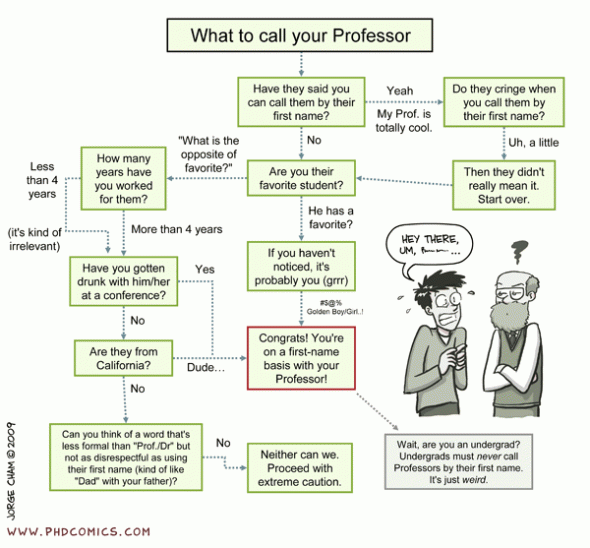
\includegraphics[scale=0.5]{files/c5.png}
\end{center}

If you're reaching out to a professor for the first time,  address them as Prof. or Dr. Lastname (if they do not have a PhD, then use Prof.). Many international students use Prof. or Dr. FirstName LastName, but this can come across as if you're simply copying and pasting names. So just stick with Prof. or Dr. Lastname.  Using Prof. is generally the safest option.

Furthermore, do not use Mr., Mrs., Ms, or Miss. This happens rarely, but I have seen  new students (e.g., undergraduate freshmen in the US) sometimes use these, which are used in K-12 schools but not in higher education.

Moreover, do not call the prof. by their first name at first.  As you become more familiar with your prof and depending on their preferences, you may transition to addressing them by their first name.
For example, I prefer that my students and colleagues call me Vu. Some students call me \emph{Dr. Vu}, which I find a bit amusing but am totally fine with it.

\begin{commentbox}[DK:]
  I was amused to read this as if I recall correctly, you never called me by my first name when you were at UNM. You always called me Prof. And, many times, I would jokingly call you back as Prof. Vu.
  \tcblower
  \textbf{Vu}: Yes, for some reason I enjoy calling you ``Professor'' (without appending a last or first name).  The use of Prof. Vu may have foreshadowed my future in academia.
\end{commentbox}

Note that in some universities the formal title Dr. Lastname is preferred over Prof. Moreover, be aware that not all faculty members may hold a PhD, in which case using Prof. Lastname is a suitable alternative. 	You just need to observe and follow the conventions at your particular institution. One way to determine how to address a professor is to observe how they sign their emails or how they introduce themselves in class. For example, I introduce myself as ``Vu'' in class.



\paragraph{Referring to professors you know} When referring or talking about a prof (e.g., your mentor) that you know, you can just informally use their names if they are OK with it as mentioned above (or Dr./Prof., if you want to be formal). You can also include their institution if it makes it more precise.  For example, I can say:  \emph{``I did my postdoc with Jeff Foster at Univ. of Maryland''}.

Do not include ranking (e.g., Assistant, Associate, Scientist, ...) when referring to someone. I see many international students include a lengthy title of people they know, e.g., \emph{I am advised by Asst. Prof. X, and I also collaborate with Distinguished Scientist Y}.  This is \emph{not necessary} and makes it look like you're trying to show off your connections. These nuances represent some cultural differences that you may encounter and will gradually adapt to. More on cultural differences in \autoref{sec:cultural}.


% \section{Having fun during a PhD?}
% PhD students \emph{and faculty} probably find it amusing about the notion that students, especially international ones, can genuinely enjoy their PhD studies. In fact, after reading posts after posts on VietPhD.org on how PhD students are commonly mistreated, stressed, it seems being miserable is a norm during a PhD study.

% There are many advice on surviving PhD that you can follow. But here I just list a few that works for me and what I advice my students to do.\tvn{TODO}




% \section{Will I be miserable during my a PhD?}\label{sec:happy}
% There are many stories of how students are mistreated, stressed, and miserable. Issues including bad relationships with professors, conflicts with co-authors and lab mates, feeling discriminated against (e.g., because you're an international student), \emph{do} exist, and it is good to be aware of those.  However, in reality, there are many good mentors, supportive lab mates and departments, and so on.  So don't let social media make you feel pessimistic and deter your quest to advance knowledge.

\appendix
\chapter{Glossary}\label{sec:glossary}

\begin{description}

  \item[ABD] All But Dissertation. A PhD candidate who has finished all course work and exams and only needs to write and defend their dissertation.

  \item[Adcom \autoref{sec:evalapps}] Admission Committee. The group of faculty members who review applications and make admission decisions.
  
  \item [Adcom members \autoref{sec:evalapps}] Faculty members who are part of the admission committee. These are the people who review applications and make admission decisions.
  
  \item[Adcom chair \autoref{sec:evalapps}] The faculty member who leads the admission committee. This person is often not involved in individual admission decisions but oversees the process (e.g., resolve disputes, ensure fairness).
  
  \item[Adviser/Superviser]: A faculty member who guides and mentors a PhD student throughout their research. This person typically plays a crucial role in a student's academic journey. In the US, the term ``adviser'' is more commonly used than ``supervisor''.
  
  \item[Cohort] A group of students who start a program at the same time and take classes together. You should get to know your cohort as they will be your colleagues and friends during your PhD.
  
  \item [Deferred Admission] An option allowing admitted students to postpone their start date, typically by one year.
  \item [Diversity Statement] A document sometimes required in applications where applicants describe their contributions to diversity and inclusion, or how their background adds to the diversity of the academic community. This document is often required for faculty positions, but some universities also require it for graduate admissions. Note that you do not need to be from an underrepresented group to write a diversity statement.
  
  \item[Domestic Student] A student who is typically a US citizen or permanent resident (``greencard holder'').
        But sometimes it can also refer to students who did their undergrad (or MS) at a US university.

  \item[Field or Area] A specific research area, e.g., Machine Learning, Computer Vision, Software Engineering, etc.
  
  \item [In-state vs. Out-of-state] In-state tuition is the tuition rate for students who are residents of the state where the university is located. Out-of-state tuition is the tuition rate for students who are not residents of that state. In-state tuition is typically much lower than out-of-state tuition. PhD students typically do not have to pay tuition as it is covered by their funding, but this might be important for MS students.
  
  \item [Ivy League] A group of eight private universities in the US known for their academic excellence and social prestige. The Ivy League schools are Brown, Columbia, Cornell, Dartmouth, Harvard, the UPenn, Princeton, and Yale. These schools are typically known for their undergraduate programs more than their graduate programs. Moreover, most top CS programs such as CMU, UIUC, UCSD, UWash, MIT, Stanford, are not in the Ivy League. See selecting and ranking schools in \autoref{sec:selecting-ranking-schools}.

  \item [Lab] Research Lab. A group of researchers (profs. and students) working on a common research area, e.g., a Software Engineering Lab.  Typically a lab is led by a single professor, but sometimes it can be co-led by multiple professors. For example, my lab \href{https://dynaroars.cs.gmu.edu}{DynaROARS} focuses on my own research area (software verification), but I am also part of the more general SWE Lab at Mason with other faculty in Software Engineering.



  \item[LoR] Letter of Recommendation. A letter written by a professor or supervisor that assesses your qualifications and potential for graduate study (\autoref{sec:lor}).

  \item[Major] A student's primary field of study, e.g., Computer Science, Electrical Engineering, Mathematics, etc. Often used in the context of undergraduate studies (e.g., ``what was your major in undergrad?'').

  \item[MS \autoref{sec:msrequirement}] Master of Science. A graduate degree that typically requires 2 years of study.

  \item[Open House \autoref{sec:accepted}] An event where admitted students visit the university to meet faculty, students, and staff, and learn more about the program. This is a great opportunity to get a feel for the university and the department and decide if it is a good fit for you.
  
  \item[Q1 Journal] Commonly mentioned by international students to refer to top-tier journals in CS.  This is not a standard in CS in the US (which often focuses on confs. rather than journals), and many CS faculty in the US might not know what this means.  If you want to refer to top-tier journals, you should mention the specific journals, e.g., TSE in Software Engineering.
  
  \item[SOP] Statement of Purpose is a document written by yourself to explains your research interests, background, and reasons for applying to a PhD program (\autoref{sec:sop}).

  \item[RA and TA] Research Assistantship (RA, \autoref{sec:ra}) is a funding where you work on a research project for a professor. Teaching Assistantship (TA, \autoref{sec:ta}) is a funding where you help a a professor with teaching (e.g., grading assignments).

  \item[TOEFL/IELTS] Test of English as a Foreign Language. A standardized test to measure the English language ability of non-native speakers.
  \item[GRE] Graduate Record Examination. A standardized test that is an admissions requirement for many graduate schools in the US. However, it is not required for most CS PhD programs (\autoref{sec:standard-tests}).

  \item [PI]  Principal Investigator is lead researcher on a grant or research project, e.g., a PI on an NSF grant.  Prospective students often use this term to refer to a professor they are interested in working with.  However, we do not use it this way in academia, e.g., ``who is your PI?'' might only make sense to fellow Reddit applicants, but might not be understood by others, ``who is your adviser?'' is what you want to use.
    \item[STEM] Science, Technology, Engineering, and Mathematics. A term used to group together these academic disciplines. CS is considered a STEM field.
  \item[URM] Underrepresented Minority. Refers to groups that are underrepresented in higher education, e.g., Black, Hispanic, and Native American students.
  \item[NSF] National Science Foundation. A US government agency that supports research and education in science and engineering. NSF is a major source of funding for RAs in CS research. There are other agencies that support RAs but they might require US citizenship or permanent residency.
    
  \item [R1/R2 Universities] Research 1 (R1) universities are universities with the highest level of research activity. R2 universities have a high level of research activity but not as high as R1 universities.  R1 universities are typically larger, and have more funding and resources for research.  R2 universities are also good but might have fewer resources and funding.
  
    \item [Rolling Admission] Applications are reviewed as they are received (instead of all at once after the deadline), and decisions are made throughout the admission cycle.  Rolling admission is more common for MS programs and less common for PhD programs (e.g., at Mason, MS is rolling and PhD is not).

  \item [Top-tier conferences and journals] These are the most prestigious venues for publishing research in CS.  For example, in Software Engineering, top-tier conferences include ICSE, FSE, and ASE and top-tier journals include TSE and TOSEM.  Publishing in these venues is highly competitive and prestigious, and can significantly improve your chances of getting admitted to a good PhD program.

        \item [Stipend] A fixed regular sum paid to students as part of their funding package (i.e., salary). This is typically paid monthly or bi-weekly.  Stipend is typically paid to PhD students and not MS students.
  \item[REU] Research Experience for Undergraduates. A program funded by the NSF to provide research opportunities for undergraduate students.
    \item[OPT] Optional Practical Training. A program that allows F-1 students to work in the US for up to 12 months after graduation.
  \item[CPT] Curricular Practical Training. A program that allows F-1 students to participate in internships or practical training that is an integral part of their academic curriculum.
  \item[F-1] Student Visa. A visa that allows international students to study full-time at an accredited institution in the US.
  \item[F-2] Dependent Visa. A visa that allows the spouse and children of an F-1 visa holder to live in the US.
\end{description}

\chapter{Visa for International Students}\label{sec:visa}

\epigraph{\vspace{-0.2in} I didn’t do it. Nobody saw me do it. You can’t prove anything!}{\textsc{The Simpsons}}


% \begin{center}
%     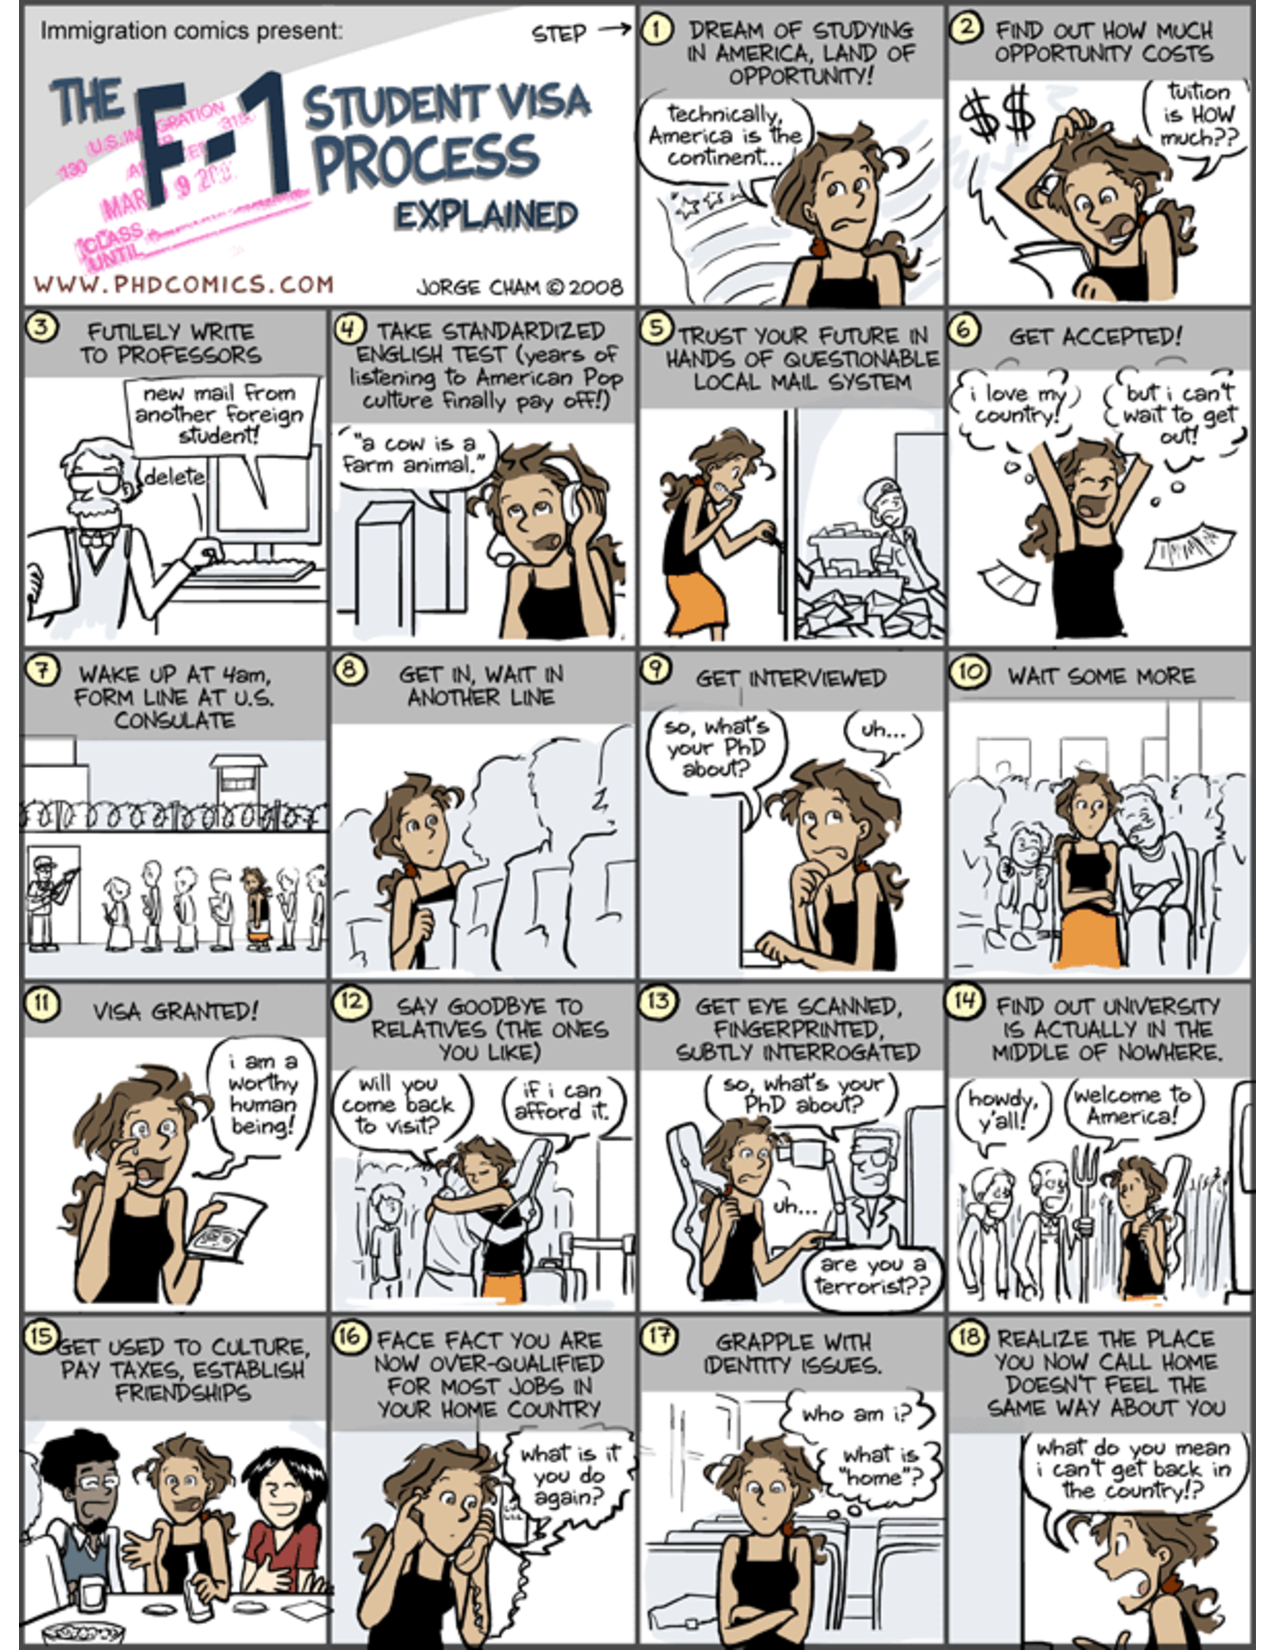
\includegraphics[scale=0.8]{files/visa.pdf}
% \end{center}

For international students pursuing a PhD in the US, \textbf{F-1} is the main visa that allows a student to study full-time at an accredited institution.  Here are some key points about the F-1 visa:

\begin{itemize}
\item \textbf{Employment:} You are allowed to work on-campus for up to \textbf{20 hours per week during the academic year} (because you still need to take classes) and \textbf{full-time} (typically 40 hrs) during official school breaks (e.g., summer and winter breaks). Off-campus employment requires authorization, which can be obtained through CPT and OPT programs described below.

\item \textbf{Curricular Practical Training (CPT):} CPT allows you to participate in internships or practical training that is an integral part of their academic curriculum. CPT must be related to your field of study and can be full-time or part-time. It requires prior authorization from your university and must be completed before graduation.

\item \textbf{Optional Practical Training (OPT):} OPT provides up to 12 months of work authorization for students before or after completing their degree. For students in STEM fields, there is an additional 24-month extension available. OPT requires prior application and approval from USCIS.

\item \textbf{Full-time Enrollment:} You must maintain full-time enrollment status during the academic year. This means taking a minimum number of credits each semester, as defined by your program. Dropping below full-time status can result in loss of visa status.
\end{itemize}

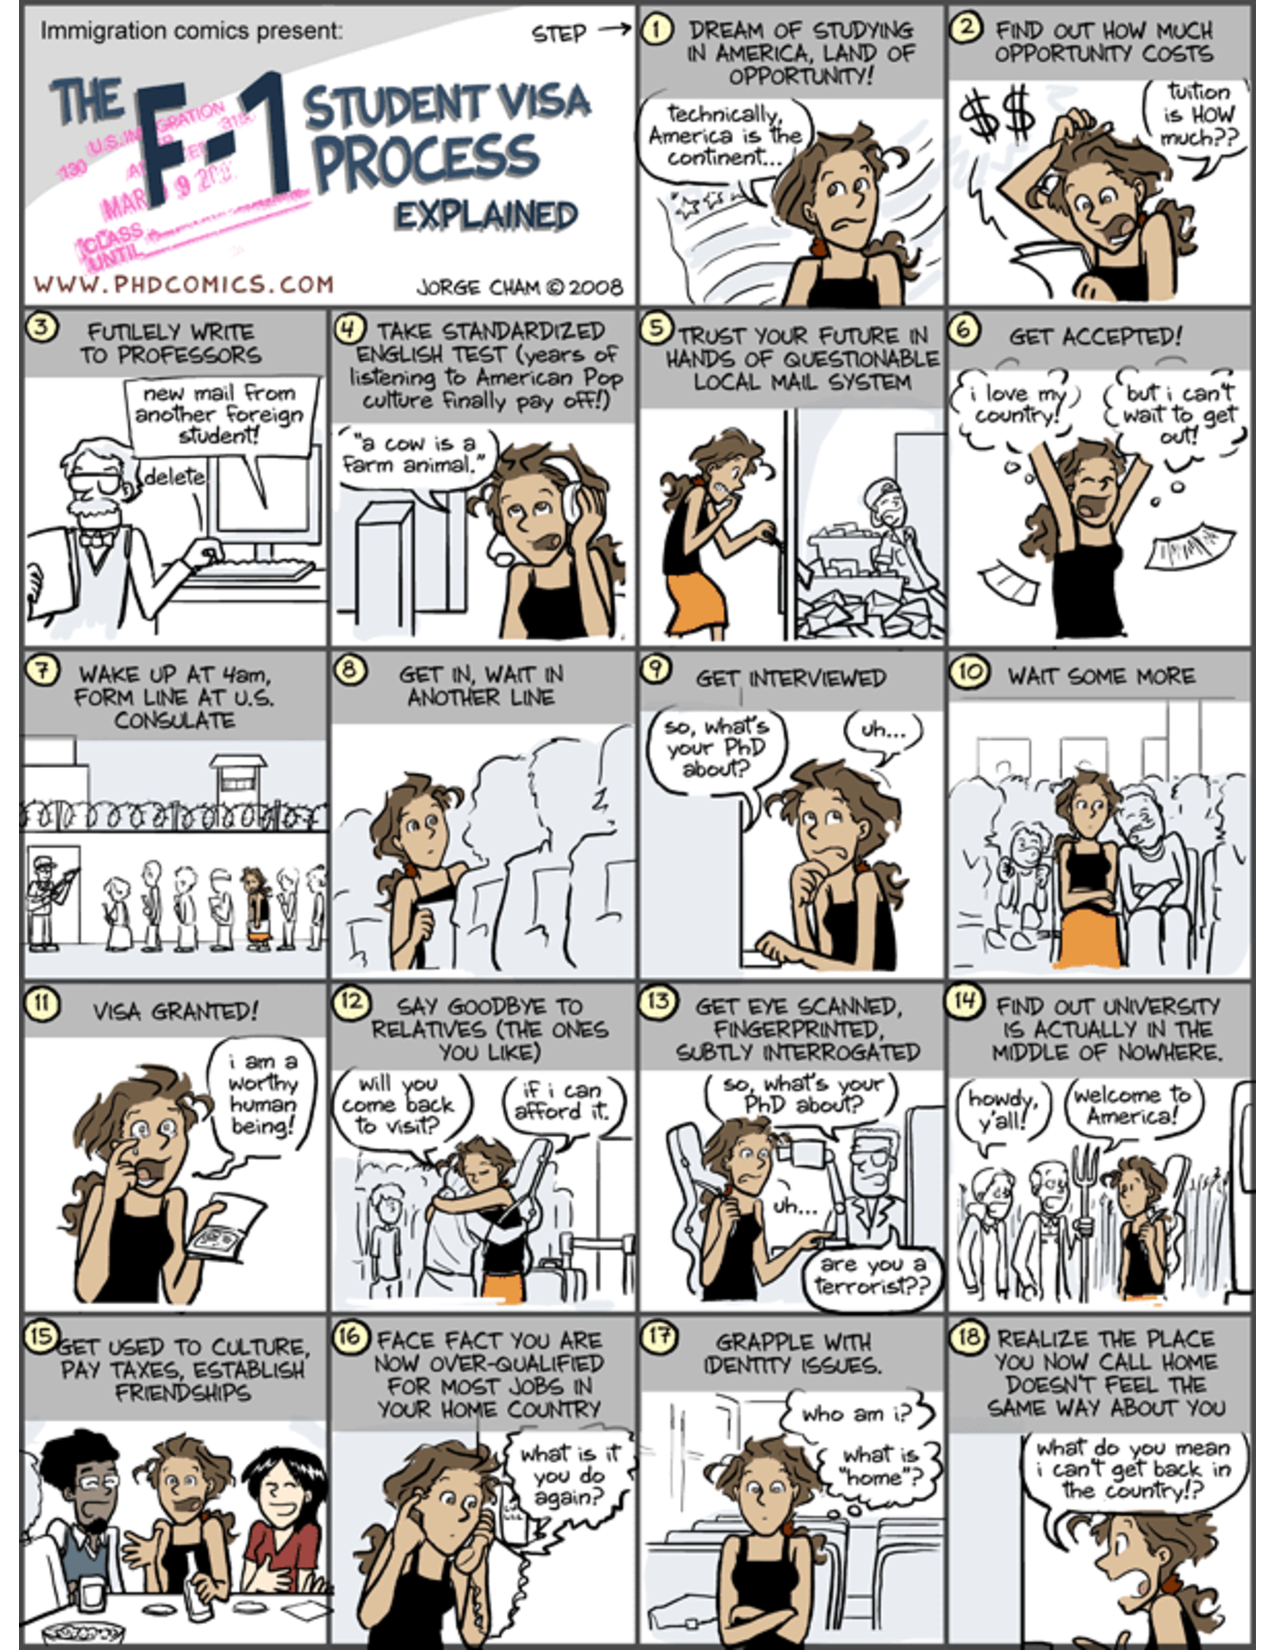
\includepdf[pages=-]{files/visa.pdf}


\section{For Spouses and Children}

The spouses and children of F-1 visa holders can enter the US under the F-2 visa status. The F-2 visa allows family members to live in the US with the following conditions:

For Spouse: 
\begin{itemize}
\item \textbf{Work Restrictions:} F-2 spouses are not permitted to work in the US.
\item \textbf{Education:} They can study part-time but cannot enroll in full-time degree programs.
\end{itemize}
For Children:
\begin{itemize}
\item \textbf{Education:} F-2 children can attend K-12 schools but cannot pursue higher education full-time.
\item \textbf{Work Restrictions:} Like F-2 spouses, children are not allowed to work under any circumstances.
\end{itemize}
F-2 visa holders must leave the US if the primary F-1 student visa holder loses status or completes their program.

\chapter{Domestic Students}\label{sec:domestic-students}
\chapterinfo{Specific benefits and opportunities for domestic students applying to CS PhD programs.}

\epigraph{\vspace{-0.2in} I’m not a bad guy! I work hard, and I love my kids. So why should I spend half my Sunday hearing about how I’m going to Hell?}{\textsc{The Simpsons}}

Most of what is written in this document applies to both domestic\footnote{For simplicity domestic means you did your undergrad (or MS) at a US university. Different universities might have different definitions, e.g., permanent residents or US citizens.} and international students.  However, there are some differences and benefits that domestic students should be aware of and can leverage to improve their chances of admission.
\paragraph{Standing out \autoref{sec:improve-your-chance}} There are \emph{few} domestic applications compared to international ones, i.e., domestic students are the minority (\autoref{sec:urm}) in the CS PhD application pool. Many US universities want to increase the number of domestic students in their programs (and as mentioned later, there are specific fellowships and funding for domestic students).
That makes you stand out and can help your case.

\paragraph{Fee Waiving} Some schools might offer application fee waivers for domestic students.  You should check with the school you're applying to.

\paragraph{School \autoref{sec:your-school}} Adcom already knows about your school, which is a plus (see \autoref{sec:your-school}). You are also more familiar with the US education system and culture (so hopefully you are aware of the cultural issues listed in \autoref{sec:cultural}).

\paragraph{Standard Tests \autoref{sec:standard-tests}} You do not need to take TOEFL or IELTS because you already did your undergrad (or MS) at a US university.  You might also be more comfortable communicating in English, e.g., contacting professors (\autoref{sec:contact}).

\paragraph{Transcripts} You do not need to get your transcripts evaluated/translated (which can be a hassle and inaccurate).  You can just send your official transcripts directly to the school you're applying to.

\paragraph{Funding \autoref{sec:funding}} You have more opportunities for funding, e.g., through government scholarships for US citizens and permanent residents.  You can also apply to specific programs \emph{before} you start your PhD, e.g., NSF Graduate Research Fellowship Program (GRFP) and Hertz Foundation Fellowship.  These fellowships are very competitive and can significantly improve your admission chances.

\paragraph{Research Experience \autoref{sec:research-opportunities}} You might have many opportunities to do research as an undergraduate, e.g., through REUs and internships at your undergrad university.  Highlight such experience in your application.

\paragraph{Open House \autoref{sec:accepted}} It is easier for you to attend open house events in person.  This can help you make a better decision on which school to attend.

% \begin{domesticbox}[Domestic students:] If you're a domestic student, you have several advantages in your application.   You also have more opportunities for funding, e.g., through government scholarships for US citizens and residents. Finally,
% \end{domesticbox}

\chapter{MS Admission}\label{chap:ms}
\chapterinfo{MS focuses on coursework and prepares you for \emph{industry}, while PhD focuses on research and prepares you for academia or research.}

While both MS and PhD programs are graduate degrees, they are \emph{very different} in terms of objective, admission requirements, course requirements, duration, and funding. This section discusses the differences and provides guidance on applying to MS programs.

\section{Differences between PhD and MS}\label{sec:phd-vs-ms}


\begin{table}
    \caption{MS vs. PhD}\label{tab:phd-vs-ms}
    \centering
    \small
    \begin{tabular}{c|c|c}
    \toprule
    \textbf{} & \textbf{MS} & \textbf{PhD} \\
    \midrule
    Objective & Industry & Research \\
    Admission Req & Research experience & No research experience \\
    Coursework Req & Yes & Yes (research is much more important)  \\
    Duration & 2 years & 5--7 years \\
    Adviser Req & No & Yes \\
    Funding & No & Yes \\
    \bottomrule
    \end{tabular}
  \end{table}

\autoref{tab:phd-vs-ms} summarizes the main differences between MS and PhD programs:
\begin{itemize}

  \item Objective: an MS is typically to prepare you for \emph{industry}, while a PhD is to prepare you for research and academia. Some MS has thesis option but the research is much lighter compared to a PhD.

  \item Admission requirements (\autoref{sec:ms-admission}): MS also requires a good GPA, LoRs, SOP, and test scores, but research experience is not required.  PhD requires all of these, but research experience is a must.
  
  \item Course requirements: MS has a specific number of courses (typically can be done in 2 years). You graduate with an MS when you're done with the courses. PhD also has coursework requirements (typically taken in your first 2 years as mentioned in \autoref{sec:time}) but focuses on research after that.  You graduate with a PhD when you have done enough research and written a dissertation, which usually takes much longer time than coursework.
  
  \item Duration: an MS typically takes 2 years while a PhD takes 5--7 years (or even longer).  Many students get an MS along the way to a PhD, e.g., after finishing the 2-year course work.
  
  \item Adviser: MS students typically do not have an adviser (if you do thesis option then you will have one), while PhD students need an adviser who guides them in their research.
  
  \item Funding: MS is typically \emph{not funded}, while PhD is (\autoref{sec:funding}). See \autoref{sec:ms-funding} for more details on MS funding.
  
\end{itemize}

\section{MS Admission}\label{sec:ms-admission}

In most cases MS CS programs are much less competitive than PhD programs, i.e., you're likely to get in if you can afford it. Many think of MS programs as a \emph{cash cow} because students are often not funded and have to pay tuition. 

While admission requirements are similar to PhD programs (e.g., GPA, SOP, LORs), research is not a focus in MS programs. In most cases, the main requirements are that you have sufficient background in CS, e.g., through your undergrad degree. This does not mean MS programs are easy to get admitted, but the requirements are much lower compared to PhD programs.

\subsection{Admission Committee}\label{sec:ms-adcom}
MS admission also involves an adcom that reviews applications and makes admission decisions. However, MS admission is typically rolling, i.e., they review applications as they come in and make decisions throughout the admission cycle.  Moreover, unlike PhD that has multiple reviewers for each application, an MS application typically involves only one reviewer and does require much time to review compared to a PhD application (\autoref{sec:ievaluate}). 

\begin{commentbox}[Vu:]
    Mason has a very large the number of MS students in CS (1000+ MS vs 200 PhDs). In contrast, other similar size universities often have much smaller MS CS programs (or none). Location plays an important role as GMU is close to DC with many developer professionals who want to get an MS, which are often covered by their employers.  Our MS program is geared towards working professionals, e.g., all of our MS courses are offered in the evening and online.
    \\
    
    The CS department has three separate committees for MS admission: MS in CS (the traditional one, which is the largest), MS in Software Engineering (SWE), and MS in Information System. 
    Each committee has its own chair and members. For example, I am often in the MS SWE adcom, which has about 3 adcom members (including the chair who also does the review). 
\end{commentbox}



%Third, adcom members can involve both teaching and tenure-line faculty (\autoref{sec:faculty-types}).


\subsection{Application Materials}

You typically need to submit the similar materials as in a PhD application, e.g., transcripts, LoRs, SOP, and test scores.  However, research experience is not required, and LoRs can be from anyone who can speak about your academic or working abilities. Moreover, your SOP should focus on your academic and work background, why you want to get an MS, and how the program fits your goals. As with PhDs, GREs are often not required. Some MS programs do not even require LoRs or SOPs.  

\paragraph{Undergrad Background and GPA} Since research is not required, your undergrad background is more important in an MS application.  You should have a strong background in CS, e.g., through your undergrad degree.  GPA is also important, as it is often used as a filter for MS applications.

\paragraph{SOP} Your SOP should explain why you want to get an MS, how the program fits your goals, and why you're a good fit for the program.  You don't need to mention about working with specific professors unless you want to do a thesis option. You still need to customize it for each school (e.g., you picked GMU due to its strong SWE program or the DC area has many job opportunities).

\paragraph{LoRs} Unlike PhDs, your LoRs do not need to be from professors or talk about research experience. Many MS programs do not even require LoRs.

\paragraph{Test Scores} GREs are often not required for MS applications.  However, some schools might still require them, and you should check with the school you're applying to.  If you have a low GPA, a high GRE score can help offset that. As with PhD, English proficiency tests (TOEFL/IELTS) are required for international students.

\subsection{Funding}\label{sec:ms-funding}
Unlike PhD programs, which often have funding (\autoref{sec:funding}), MS students are typically not funded. The reason is because MS students do not focus on research and thus are not funded through RA and PhD students have priority for TA positions. 
\begin{itemize}
\item[\textbf{RA}] Profs. are not willing to take MS students as RAs because they are not around long enough to be productive. It can take a while for a student to get up to speed and start being productive, and by that time, they are about to graduate. Moreover, the goal of most MS students is to get a job, not to do research, so they are not as motivated to do research.

\item[\textbf{TA}] MS students are typically not given TA positions because PhDs are given priority. Many depts. do not have enough TAs for PhD students and so they cannot afford to give them to MS students.
\end{itemize}

However, there are always exceptions, e.g., if you have a strong background and can demonstrate that you can be productive in research, then a prof. might be willing to take you as their RA.
Moreover, some schools have TAs for MS students, and you can apply for these positions. For example, Mason CS has quite a few TAs for MS students; my courses in the past two years have MS TAs.

\section{Selecting and Ranking Schools}\label{sec:selecting-ranking-schools-ms}
%\sectioninfo{How to select and rank MS programs in CS.}

Because of the differences between MS and PhD programs, you should consider different factors when selecting and ranking MS programs. For example, you might want to consider factors such as location, industry connections, and job placement instead of research areas and advisers (\autoref{sec:schoolsandprofs}).

\begin{itemize}

\item \textbf{Location:} In addition to living in a place you like (e.g., warm weather, historical city, etc.), you should also consider the job opportunities in the area.  For tech industry, consider MS programs in tech hubs like the Bay Area and Seattle. For government jobs, look at schools in the DC area.  For example, many students at Mason work for the government or defense contractors in the DC area and take classes in the evening or online.

\item \textbf{Industry Connections:} Universities often have strong connections with local companies and can help you get internships and jobs. For example, Microsoft and Amazon look for students in the Washington area while  Google and Facebook recruit those in the Bay Area.  Mason students natural get jobs from the government, defense contractors, and Amazon, whose 2nd HQ is in Arlington.

\item \textbf{Ranking:} Unlike PhD programs where the adviser and research are perhaps the most important factor, in MS programs the ranking of the school is more important.  Thus, you should consider the ranking of the school in CS, especially in the specific area you're interested in.  For example, if you're interested in software engineering, you might want to consider schools with strong SWE programs. 

\item \textbf{Living Cost:} MS students are typically not funded, so living cost can be a big factor. You should consider the tuition and living expenses of the area. Note that sometimes living costs, e.g., renting, seem scary at first but students often find way to make it work, e.g., by sharing an apartment with other students.

\end{itemize}


\chapter{Research Opportunities}\label{sec:research-opportunities}
\chapterinfo{How to get research experience as an undergrad.}

\epigraph{\vspace{-0.2in} Kids, you tried your best and you failed miserably. The lesson is: never try.}{\textsc{The Simpsons}}



\begin{center}
    
\includegraphics[scale=0.5]{files/phd100404s.png}
  \end{center}

As discussed in \autoref{sec:research-experience}, having a successful research experience can greatly strengthen a PhD application. Research experience gives you opportunities to try out research, determine what research area you're interested in, publish papers (\autoref{sec:research-experience}), connect with researchers, and get strong LoRs (\autoref{sec:lor}). This section provides some guidance on how to gain research experience as an undergraduate student or student at a smaller college where research opportunities might be limited.

\paragraph{Locally} Start looking for research opportunities at your institution.
If you did well or liked a class, you can check with the professor of that class for research opportunities.
You can also go to the department directory and then professors' websites and see if they are looking for undergraduate researchers.
Even if they say they are looking for graduate students, you can still contact them and ask.

There might be also special programs for undergraduate research from the university, e.g., Mason has the OSCAR program, UNL has UCARE, and NSF has REUs (for US citizens and permanent residents).

You can also take honor thesis or independent study courses with a professor.  This is a good way to get research experience and also get a LoR from the professor.  You can also ask your academic adviser or other faculty members for suggestions.  Finally, you can also ask your peers who are already doing research.  Use the method described in \autoref{sec:contact} to contact professors


\begin{commentbox}[Vu:]
    I enjoy working with undergrads (e.g., I have mentored over 15 undergrads) and always actively recruit.
    I often get undergraduate researchers through my classes, e.g., asking students who did well in my class if they are interested in research.  Occasionally I was introduced to students by other students or faculty.\\

    While most undergrads are understandably not super productive in research, some are and I have published multiple papers with them.  I also have written strong LoRs for them and have helped them get into good PhD programs.

    \tcblower
    At Mason we pay undergrads about \$15/hr and about 10 hrs/week. This is flexible and can be increased as needed.
\end{commentbox}

\paragraph{Online Research Communities and Open Source Contributions} Places such as GitHub offer many research opportunities, even though they might not appear so (e.g., they do not explicitly mention research).
In many cases, professors or research labs put their projects on GitHub. For example, my research group, \href{https://github.com/dynaroars/}{Dynaroars}, has many open-source projects that undergrads can contribute to.

By contributing code, fixing bugs, implementing new features, or providing documentation, students can gain practical research experience and interact with experienced developers and researchers in the field. Not only you gain research experience, but you might be able to get a LoR from the project maintainer, and you should write about this experience in your SOP (\autoref{sec:sop}.)

\paragraph{Virtual Research Opportunities} This is less common but several places offer virtual internships and research programs aimed at providing hands-on research experience. These programs often involve working remotely under the guidance of experienced mentors and collaborating with a team of fellow researchers. For instance, \href{https://docs.google.com/forms/d/1btIwt4HwjyKMOUk-EMy3rbkfWzFxv2lNrMm_zkd0pA4/viewform?edit_requested=true}{UIUC+ Summer Undergraduate Research in Software Engineering}  offers an unpaid remote internship for software engineering students all over the world to collaborate with mentors from University of Illinois at Urbana Champaign.

% \paragraph{Online Conferences and Workshops}: Attending online conferences and workshops is another way to gain exposure to cutting-edge research and establish connections with experts in the field. Many conferences now provide virtual participation options, enabling students to access research talks, poster sessions, and panel discussions and sometimes access designated chat rooms or networking events where participants can engage with researchers, ask questions, and seek potential research collaborations. By creating profiles, joining relevant research groups, and participating in discussions, students can connect with established researchers, contribute to ongoing projects, and potentially collaborate on publications or research proposals as they provide access



\chapter{Cultural Differences}\label{sec:cultural}

\epigraph{\vspace{-0.2in} Ay caramba!}{\textsc{The Simpsons}}


This section lists some general cultural issues that students, especially international ones, might want to pay attention to.

% \paragraph{Diversity} US universities prioritize diversity and inclusion. Students need to respect and appreciate varied opinions, backgrounds, and cultures. Unlike some countries where certain voices are marginalized, in the US, all perspectives are valued equally (especially at universities). Racism or discrimination will have serious consequences, including academic and disciplinary actions.


\section{Academic Integrity (Cheating and Plagiarism)}

Plagiarism and cheating (e.g., exams and assignments) are a BIG no-no in the US.  If you're caught cheating, you will face serious consequences and likely be expelled from the university (e.g., after the second time at Mason).   This is quite different from many international countries where cheating is common and often tolerated.  Faculty is extremely good at detecting cheating (we have been dealing with these situations so many times over so many years), and \emph{will} report cheating cases.  In short, whatever you do, don't cheat---not worth it.

Here are the typical steps: (i) a faculty suspecting a cheating case will report it to the Office of Academic Integrity (OAI) at the university---the report often has supporting evidence and suggested penalty (e.g., a failing grade);  (ii)  OAI will completely take over and investigate the case independently (the prof. is not involved); and (iii) OAI will make the final decision.  It is important to note that after receiving the report from your prof., OAI \emph{completely} takes over and makes its own decision.  This means begging your professor will not help because they simply are no longer involved in the case and cannot do much.

\section{Illegal Software}\label{sec:illegal-software}
 Using illegal/cracked software is very common in many countries (and even in the US). However, \emph{do not} install or use them on university computers, even those given to you by your adviser.  It is unlikely that the university will track you down, but it is the \emph{software company} that will.  They have very sophisticated tools to detect illegal software and will sue your university/department.  Imagine your department or adviser being sued for a large sum of money, and it is \emph{you} who caused it.  If you need to purchase software,  ask your adviser or the department (\autoref{sec:buying-equipment}).


\section{Costly Gifts}\label{sec:gifts} In many countries, it is customary to give professors costly gifts (e.g., expensive liquors, jewelry, or even money), often during the holidays, to show respect and appreciation.  In the US, this is can be considered \emph{inappropriate} and discouraged. 

However, if you'd like to offer small souvenir-like tokens, it's a thoughtful gesture that's appreciated. Some professors proudly display their gifts, which can come from students and colleagues (e.g., when they travel to their home countries or conferences). In summary, small gifts are fine, but avoid anything that might make your professors uncomfortable.


\section{Maintaining Good Relationships with your Profs.}
There's a misconception that in the US it's all business, with professors as bosses who pay students for their work and that lab mates are just work colleagues; and that doing nice things means expecting something in return.

However, the reality is quite the opposite. While people can be straightforward and appear ``cold'', they are also informal, friendly, and very caring (in ways that might surprise you).
With lab mates and colleagues, you will often work and go to lunch together, confide in each other, help each other navigate the academic journey, and often become lifelong friends.
With your professor(s), you can call them by their first name (\autoref{sec:address}), disagree with them and argue (and gain respect doing so), seek their help (even on personal matters), come to their houses for parties or gathering (e.g., my lab always come to my house for \href{https://photos.app.goo.gl/LFtbqQUuznq9eiL7A}{Thanksgiving}), and give them small thoughtful gifts that they put on their desks (\autoref{sec:gifts}).  
Many people maintain lifelong relationships with their professors and colleagues, staying in touch through cards, emails, and visits, even after they no longer work together.

\begin{commentbox}[Vu:]
    I maintain a close relationship with my former professors and mentors. When there is a new event in my life (or theirs), I often email them or call them, e.g., when I get married, have a new baby, new job, etc. When I was having issues at UNL and considering leaving, I talked to my PhD advisers Deepak and Steph. I think this does not bother them a bit; they are genuinely interested in knowing and helping solve these ``dramas'' in my life.
    \\
    
    I also visit my former professors when I am in their area. I meet Thang Bui (my MS adviser) at least once a year when I come back to Harrisburg to visit my parents. When Steph was in DC for a meeting, I invited her to to give a research talk at Mason. I have also collaborated with them after I graduated e.g., I recently got an NSF grant with Deepak.
    \\
    
    In short, while I am a bit closer to my former advisers and mentors than most people (e.g., I still keep in touch with my middle school teacher in Hawaii), it is always a good idea to maintain a good relationship with people who have helped or worked well with you. A simple, short email or text once in a while (e.g., a \emph{``Hi X, I heard you just got promoted ... Congrats!''}) would suffice. They will appreciate it, and you never know when you might need their help.
    
        
  \end{commentbox}
  
  \section{Miscs}\label{sec:cultural-misc}
  
  Several other common surprises for international students (and foreigners in general) in the US. Note that I skip topics involving politics, religion, tax, and racism as these happen in many countries and are not unique to the US.

\paragraph{Small talks} People often engage in small talks, e.g., about the weather, sports, or weekend plans.  This is a way to start a conversation and how social interaction starts in the US.
  
Moreover, avoid asking personal questions, e.g., about salary, age, relationship status, or health, as these are considered private.  Talking about kids' activities or schools are OK. Also, do not talk about politics or religion.  In fact, we often do not talk about these taboo subjects with our family and friends to avoid conflicts.  

Sometimes foreigners are surprised by how Americans do not talk about their personal lives, e.g., sharing details about their families, health, or relationships, and that their conversations are often not very ``deep'' or ``mind-provoking''. This is just a cultural norm about privacy and personal space.

  \paragraph{Healthcare System}  You (and your spouse) will need health insurance! Otherwise you will be charged a lot for healthcare services. However, as mentioned in \autoref{sec:funding}, your  TA/RA  will cover health insurance (and your spouse/children also get insurance or discount for it). 
  
  However, be aware that heathcare services can still be expensive even with insurance. So  know what your insurance covers and be prepared for unexpected costs.  Moreover, healthcare system has many confusing jargons such as HMO, PPO, deductibles, co-pays, and coinsurance (try take a look at the Explanation of Benefits or EoB statement you received from your insurance company). It's arguably the most complicated system in the US and even Americans often do not understand it (and politicians often exploit this to their advantage).  So do not hesitate to ask your HR or the insurance company for help.
  
  
  \paragraph{Tipping Culture} Unlike many other countries, tipping is expected for various services, especially in restaurant. So adding an extra 15--20\% to your bills is common, especially in restaurants.
  You should also tip for other services, e.g., Uber, taxi, haircuts, and hotel services.  The minimum wage for tipped employees is lower than the standard minimum wage, so tips are an important part of their income.

  \paragraph{Car Dependency} Most places in the US are highly car-dependent. If you do not have a car, you will need to rely on friends, Uber, or public transportation, which can be inconvenient and time-consuming. Many international students end up getting a driver's license, which is highly convenient and replaces many documents (e.g., ID, passport) and buying a car.


  %\paragraphP{Conversation} Americans are generally friendly and open.  However, there are certain things that we rarely talk about, e.g., salary, relationship status, or health. 
  These are considered private and should not be asked.  Also, do not talk about politics or religion in general (in fact, we do not even talk about these with our family and friends to avoid conflicts).  
  
  
  %Sometimes foreigners are surprised by how Americans do not talk about their personal lives, e.g., sharing details about their families, health, or relationships, and that their conversations are often not very ``deep'' or ``mind-provoking''. This is just a cultural norm about privacy and personal space.
  
  
  %This can be surprising for people from countries where strangers do not typically talk to each other.  Americans are also generally informal and use first names, even with people they have just met.  This can be surprising for people from countries where titles and last names are used, even with close friends.
	%\paragraph{Individualism} The strong culture of individualism in the US can be both liberating and isolating. For example, Americans are encouraged to express their opinions and pursue their goals, and are more focused on their personal rights (e.g., they do not want people do things in front of their house). 



  % \paragraph{Racism and Segregation} While some find the US to be less racist than expected, others note that racism and segregation are still prevalent, often manifesting subtly in daily life or visibly in segregated neighborhoods.

	%\paragraph{Litigiousness} The US is known for its litigious culture, where lawsuits are common, and people can be sued over seemingly minor issues. This can be surprising for newcomers used to different legal systems.


  % \paragraph{Consumerism and Scale} The US is often associated with large portions, big cars, and massive stores like Costco. The emphasis on consumption and abundance is notable.

	% \paragraph{Religious Influence} Religion, particularly Christianity, plays a more visible role in public and political life in the US compared to many other countries.


% \begin{commentbox}
%   [DK:] Here are a few items you may consider addressing: putting international students in touch with other students from their countries, assuring them that they would be picked up from airports upon their arrival and that their initial stay will be taken care of. Most universities have other resources for these, but it is worth mentioning that they would be taken care of upon arrival and can get help during the transition phase. Learning to cook was a big deal when I arrived over 50 years ago-August 1973. But things have changed as one can find many ethnic food places, a big contrast from 1973, when there were two Indian restaurants in Greater Boston area.
% \end{commentbox}


\chapter{CSRankings: Rankings of CS PhD programs}\label{sec:ranking}
\chapterinfo{CSRankings.org is a ranking system based on faculty publications at top CS conferences.}

\epigraph{\vspace{-0.2in} The whole damn system is wrong!}{\textsc{The Simpsons}}


\begin{table}[h]
  \centering
  \small
  \caption{The top 50 CS programs in the US from \href{https://www.csrankings.org}{CSRankings.org}, a ranking system  based on faculty publications at top CS conferences. (\href{https://csrankings.org}{CSRankings}, Jan. 2024). \red{$^*$} indicates that the university has \href{https://github.com/dynaroars/dynaroars.github.io/wiki/Viet-CS-Profs-US}{Vietnamese prof.} that can advise CS PhD students.}\label{tab:ranking}
  \begin{tabular}{rl|rl}
    \toprule
    1 & Carnegie Mellon & 26 & Duke University \\
    2 & Univ. of Illinois at Urbana-Champaign\red{$^*$}  & 27 & Univ. of California - Santa Barbara \\
    3 & Univ. of California-San Diego & 28 & Rutgers University\red{$^*$} \\
    4 & Georgia Institute of Technology & 29 & Univ. of California - Riverside\\
    5 & MIT                            & 30 & Pennsylvania State University  \\
    6 & Univ. of California - Berkeley& 31 & Northwestern University\\
    7 & University of Michigan - Ann Arbor\red{$^*$}   & 32& George Mason University\red{$^*$}\\
    8 & University of Washington      &33 &  Texas A\&M University\red{$^*$} \\
    9 &  Stanford University  &34&  University of Utah \\
    10 & Cornell University  & 35 &  North Carolina State University\\\
    11 & University of Maryland - College Park &  36& Ohio State \\
    12 & Northeastern University\red{$^*$} &37& University of Virginia  \\
    13 & Purdue University &38& Yale University \\
    14 & University of Wisconsin - Madison\red{$^*$} &39 & Univ. of California - Santa Cruz \\
    15 & University of Texas at Austin &40& Brown University \\
    16 & University of Pennsylvania &41 & Harvard University \\
    17 & Columbia University\red{$^*$} &42 & Boston University  \\
    18 & Princeton University\red{$^*$}  & 43& Rice University\\
    19 & New York University  & 44&  University at Buffalo\red{$^*$}\\
    20 &  University of Massachusetts-Amherst\red{$^*$} &45& University of Colorado-Boulder \\
    21 & Univ. of California - Los Angeles &46& University of Illinois at Chicago  \\
    22 & University of Southern California &47& University of Minnesota \\
    23 & University of Chicago &48& University of North Carolina\red{$^*$} \\
    24 & Stony Brook University\red{$^*$} &49& Arizona State University\red{$^*$} \\
    25 &  Univ. of California - Irvine&50& Univ. Of California - Davis \\
    \bottomrule
  \end{tabular}
\end{table}
% Virginia Tech\red{$^*$}  \\

%\autoref{tab:ranking} lists .
\chapter{History and Acknowledgement}\label{sec:ack}
\paragraph{History} This document was conceived during a lunch with a faculty at Mason.  We talked about why Mason was not able to attract good Vietnamese and other international students, despite having a much stronger CS program than many schools that these students want to go to (part of the reason is described in \autoref{sec:selecting-ranking-schools}). We wish there were a way for international students to know about PhD programs in the US.

I was also a member of the large VietPhD group on Facebook and often browse Internet forums (e.g., \texttt{Reddit/gradadmission} and \texttt{GradCafe}). There I saw many questions from students about PhD programs.  However, most participants are students in non-CS fields or not in the US, and their answers are not always accurate and can lead to more confusion. So I thought it would be useful to have a document that is specific to CS PhD programs in the US from an insider perspective.

I started writing this document in May 2023 and have been updating it since then (mostly around deadline time when I tend to procrastinate, i.e., \emph{productive procrastination}!). The document was initially intended for international students but has been generalized to all students.
I have put the source code of this document on \href{https://github.com/nguyenthanhvuh/phd-cs-us}{GitHub} so that others can contribute to it.

\paragraph{About Me} I am an associate professor in the CS dept at George Mason University (Mason). Before Mason, I was at the University of Nebraska-Lincoln (UNL). I have been in the PhD admission process at Mason and UNL for many years. This allows me to have a good understanding of the process, the challenges students face, and what faculty are looking for. I also serve as the program director of the MS program in Software Engineering at Mason (thus also have experience with MS admission---which is quite different than PhD as discussed in \autoref{chap:ms}). My personal and lab website is at \href{https://dynaroars.github.io}{dynaroars.github.io}.

Though I was not an international student, many of my students and collaborators are/were. I also mentor multiple students from Vietnam and have close colleagues and friends who were once international students. I hope to capture the diverse challenges and experiences they've faced in this document so that it can be a valuable resource for prospective international students.
Finally, my upbringing in the US provides a perspective aligned with American culture, allowing me to shed light on various issues, particularly those related to cultural differences (\autoref{sec:cultural}).




\paragraph{Acknowledgement} Many people have contributed to this work.
Profs. Craig Yu (Mason), Hakan Aydin (Mason), 
Xiaokuan Zhang (Mason), Hung Le (UMass), and Deepak Kapur (UNM) provided valuable input in the early version. Other Mason faculty members also have provided feedback and contributions.  Many students including Didier (Mason), Thanh (Melbourne), and Dat (Melbourne) have contributed valuable questions and feedback. 

Also thanks to NSF for encouraging faculty to be creative in research and education, which allows me to write this document. 

\textbf{Thank you!}

%\bibliographystyle{abbrv}
%\bibliography{demystify.bib}

\end{document}



